% Main entry point; all document inputs and graphics are local to doc/.
\documentclass[11pt,oneside,openany]{book}
% Ordinary LaTeX packages; no external SWMF style or AGU bibliography style.
\usepackage[T1]{fontenc}
\usepackage{iftex}
\ifPDFTeX
  \usepackage[utf8]{inputenc}
\fi
\usepackage{lmodern}
\usepackage[letterpaper,margin=0.9in,headheight=15pt]{geometry}
\usepackage{graphicx}
\usepackage{amsmath,amssymb}
\usepackage{booktabs,longtable,tabularx,array}
\usepackage{xcolor}
\usepackage{listings}
\usepackage{microtype}
\usepackage{hyperref}
\usepackage{bookmark}
% Use the standard url package on every machine, with one consistent wrapping
% policy. Retain its punctuation breaks and add ASCII letters/digits so long
% source names, test identifiers and registry hashes fit table columns. These
% formatting rules preserve every printed character and hyperlink target.
\usepackage{url}
\makeatletter
\g@addto@macro\UrlBreaks{%
  \do\a\do\b\do\c\do\d\do\e\do\f\do\g\do\h\do\i\do\j\do\k\do\l\do\m%
  \do\n\do\o\do\p\do\q\do\r\do\s\do\t\do\u\do\v\do\w\do\x\do\y\do\z%
  \do\A\do\B\do\C\do\D\do\E\do\F\do\G\do\H\do\I\do\J\do\K\do\L\do\M%
  \do\N\do\O\do\P\do\Q\do\R\do\S\do\T\do\U\do\V\do\W\do\X\do\Y\do\Z%
  \do0\do1\do2\do3\do4\do5\do6\do7\do8\do9}
\makeatother
\Urlmuskip=0mu plus 1mu\relax
\hypersetup{colorlinks=true,linkcolor=blue!45!black,urlcolor=blue!45!black,
 citecolor=blue!45!black,bookmarksnumbered=true}
\setcounter{tocdepth}{1}
\setcounter{secnumdepth}{2}
\setlength{\emergencystretch}{3em}
\setlength{\parskip}{0.35em}
\setlength{\parindent}{0pt}
\newcolumntype{L}[1]{>{\raggedright\arraybackslash}p{#1}}
\newcommand{\code}[1]{\texttt{\small\detokenize{#1}}}
\newcommand{\source}[1]{\par\smallskip{\small\textbf{Source guide: }\path{#1}}\par}
\newcommand{\scope}[1]{\par\smallskip\noindent
 \fbox{\begin{minipage}{0.94\linewidth}\small\textbf{Scope.} #1\end{minipage}}\par}
\lstdefinestyle{amps}{basicstyle=\ttfamily\footnotesize,columns=fullflexible,
 keepspaces=true,showstringspaces=false,breaklines=true,breakatwhitespace=false,
 frame=single,framerule=0.25pt,rulecolor=\color{black!25},
 backgroundcolor=\color{black!2},xleftmargin=0.1em,xrightmargin=0.1em,
 aboveskip=0.8em,belowskip=0.8em,upquote=true,tabsize=2}
\lstset{style=amps}

\hypersetup{pdftitle={AMPS User and Developer Manual},pdfauthor={AMPS development team}}
\begin{document}
\frontmatter
% The unnumbered title sheet and first front-matter page otherwise both
% acquire the Roman-page anchor "i" when titlepage resets the counter.
\hypersetup{pageanchor=false}
\begin{titlepage}
\centering
\vspace*{0.8cm}

\includegraphics[width=0.86\textwidth,keepaspectratio]{AMPS_clean_sweep_white.jpg}
\vspace{1.2cm}
{\Huge\bfseries AMPS\par}
\vspace{0.4cm}
{\Large Adaptive Mesh Particle Simulator\par}
\vspace{0.8cm}
{\huge User and Developer Manual\par}
\vspace{0.8cm}
{\large Core, applications, physics, coupling and validation\par}
\vfill
{\large AMPS development team\par}
\vspace{0.4cm}
{Repository documentation edition: 10 November 2026\par}
\vspace{0.6cm}
\begin{minipage}{0.85\textwidth}\small
This manual describes the source tree and bounded validation available at the
edition date. A documented capability is not a claim that every combination of
algorithms, inputs, machines or scientific applications has been qualified.
\end{minipage}
\end{titlepage}
\hypersetup{pageanchor=true}
\chapter*{How to use this manual}
\addcontentsline{toc}{chapter}{How to use this manual}
Start with Chapters~\ref{ch:introduction}--\ref{ch:inputs} for a first run.
Choose the physics and boundary chapters before choosing numerical controls.
Chapter~\ref{ch:tests} explains evidence and test execution;
Chapter~\ref{ch:examples} provides executable examples with explicit oracles.
Developers should also read Chapters~\ref{ch:architecture}, \ref{ch:output}
and~\ref{ch:development}. Paths in code listings are relative to the AMPS root
unless a different working directory is shown.

\paragraph{Evidence vocabulary.}
\emph{Implemented} means code exists. \emph{Verified} means a stated numerical
or software contract has independent evidence. \emph{Scientifically validated}
requires an appropriate physical reference or observations, error estimates
and the declared domain of validity. These terms are deliberately distinct.
The test catalog lists registered intent; an actual run receipt records execution.
Historical numerical results in this manual are dated snapshots.

\paragraph{Build independence.}
The manual compiles from a copy of this directory with a suitable TeX engine;
neither an AMPS executable nor SWMF, SPICE, a generated build tree or remote
figures are required. The accompanying README gives the exact commands.
\tableofcontents
\listoftables
\mainmatter
\chapter{Introduction and model scope}\label{ch:introduction}
\section{What AMPS solves}
AMPS is a kinetic simulation framework for rarefied gas, neutral and charged
particle populations on adaptive meshes. Applications use its particle
records, transport, stochastic reactions/collisions, surface interactions,
sampling and distributed data structures. Depending on configuration, fields
are prescribed, coupled from another model, or advanced by supported PIC
solvers. The same framework supports planetary exospheres, comet comae and
dust, magnetospheric particles and heliospheric transport.

AMPS can run standalone or as an SWMF component. A standalone application
owns its outer lifecycle; SWMF supplies component communicators, scheduling
and coupling epochs through wrappers. Shared numerical machinery does not
make the scientific assumptions of one application valid in another.

\section{Choose the physical problem first}
A useful run description states the species, phase-space representation,
geometry/frame, initial and external boundary conditions, injection rate and
velocity law, force model, reaction network, surface physics and observable.
Then state mesh, time-step, particle-weight and sampling policies. If any
required physical information is absent, resolve it before running: numerical
convenience is not a physical closure.

For example, a neutral Enceladus parent-loss calculation can have H2O and CO2
particles while allocating no photoproducts and using no plasma. A comet
network can instead produce daughters with recoil and internal energy. A
field-line SEP model and a full 3-D charged-particle mover have different
transport approximations. A source-free analytical CME background test cannot
qualify particle acceleration or a full downstream plasma volume.

\section{Four kinds of evidence}
\begin{enumerate}
\item Structural checks verify grammar, registration, data identity and
supported configuration. They need not evolve any physical state.
\item Numerical verification compares an algorithm with independent equations,
manufactured solutions, conservation or convergence.
\item Regression testing detects change relative to reviewed fixtures and can
include a full configure/build/run/output path.
\item Scientific validation compares the declared physical model with relevant
laboratory, observational or independently justified physical reference data.
\end{enumerate}
These layers complement each other. A model can conserve particles while
using the wrong source law; it can reproduce a fitted observation without
independently validating that source. Reports must preserve the distinction.

\section{Reading and operating conventions}
Bare dimensional values in modern application runtime keys generally use the
SI units stated by the owner; older generators and external tables can have
explicit different units. The applicable input parser is authoritative.
A path shown in a command is relative to the repository root unless a working
directory is declared. Placeholders must be supplied by the operator.
The documented test commands use a required machine profile rather than
hard-coded compiler/kernel paths. Native build examples require an idle
checkout and a clean generated build as explained next.
\source{src/README.md; src/pic/README.md; src/test/README.md}

\chapter{Installation, configuration and execution}\label{ch:installation}
\section{Prerequisites and source distribution}
Use an existing authorized checkout or source archive with its maintained
shared libraries, inputs and test fixtures. Preserve the supplied directory
layout. This edition does not prescribe an obsolete CVS host or silently
retrieve missing model data. Record the source revision and local changes
with each production build.

The native toolchain needs a compatible C++ compiler, make, Perl and MPI;
dependency-light modern contracts commonly require C++17. Python 3 runs the
global test procedure and many post-processors. A Fortran compiler and matching
MPI interface are required for SWMF and selected linked modules. Optional
capabilities can require CSPICE, external field libraries, numerical tables,
matplotlib/NumPy or an accelerator toolchain. Inspect the chosen application
and machine profile rather than assuming all dependencies are universal.

\section{Site configuration and application selection}
The established \path{Config.pl} workflow selects the application and site
settings. It uses \path{input/NAME.input} first and falls back to
\path{input/NAME.conf} only if the former does not exist. Initial installation
and compiler selection are site-specific; inspect \code{./Config.pl -help}
and the existing \path{Makefile.conf}. Preserve site libraries and settings.
Do not edit \path{.amps.conf} directly.

For a new compile-time application selection:
\begin{lstlisting}
./Config.pl -show
./Config.pl -application=enceladus
\end{lstlisting}
Changing the runtime .in file selects only among compiled capabilities; it
cannot change species IDs, dimension or allocated record layout.
Generated files in \path{build} or \path{srcTemp} are not the maintained
place to implement a lasting fix.

\section{Mandatory native rebuild sequence}
Before \emph{every} native AMPS rebuild, confirm the repository root and verify
that no build or test simulation is using it. In the current workspace the
root is \path{/home/vtenishe/Mars2/AMPS}. From that confirmed, idle root:
\begin{lstlisting}
# Remove only the generated root build directory.
rm -rf -- build

# Regenerate the chosen application's configuration/hooks.
./Config.pl -application=enceladus

# Use the established top-level compilation workflow.
env MAKEFLAGS="-j16" make amps
\end{lstlisting}
Some application guides explicitly stage generator hooks before make:
\begin{lstlisting}
./ampsConfig.pl -input enceladus.input -no-compile
\end{lstlisting}
Follow the selected adapter's established sequence. Do not remove source directories,
site settings, libraries or another checkout. A focused standalone compile of
a shared-model test is not a native AMPS build.

The global native test adapters perform and record this preflight under
exclusive ownership. Prefer them for reproducible verification. Do not run a
second manual Config.pl or make against their active checkout.

\section{SPICE configuration and data readiness}
SPICE-enabled applications require both the toolkit and appropriate kernels.
Configure explicit local paths through the established workflow, for example:
\begin{lstlisting}
./Config.pl -spice-path=/path/to/SPICE/cspice \
  -spice-kernels=/path/to/SPICE/Kernels
\end{lstlisting}
These paths are placeholders. A no-SPICE fixture selects
\code{-spice-path=nospice}; a component-level SPICE-off input by itself may
not remove an inherited global toolkit/link choice.
Test actual state and orientation queries for the intended target, frame and
epoch. The presence of a file with a plausible name is not proof of coverage.
Record versions/hashes and load order; never substitute an unrelated mission
ephemeris to make initialization succeed.

\section{Run directories, MPI and batch execution}
Use a fresh run directory and freeze the exact executable and inputs. Paths
inside application files may resolve relative to the input file or the run
directory; inspect the owner. Copy/include all dependent source distributions,
event files and data receipts, preserving that relationship.
A minimal launcher pattern, after preparing a complete run, is:
\begin{lstlisting}
cd /path/to/prepared/run
mpiexec -n 4 ./amps -input run.in > run.log 2>&1
\end{lstlisting}
This is a launch pattern, not a universal CLI or rank recommendation. I3 uses
\code{-i FILE -case N}; some legacy applications take no runtime file.
Choose the MPI rank flag and launcher from the site's configuration. Allocate
memory for blocks, ghosts, particles, node fields and output buffers; counts
of CPUs alone do not establish that a case fits.

A batch script should set the working directory, requested ranks/threads,
required modules and log destinations explicitly. It must retain the real
process return code. Do not assume a shell pipeline to a logging command
preserves the simulation's failure code. Use the scheduler allocation, not
an arbitrary host-specific job example from an old manual.

\section{A first verification before a science run}
Run the fast global campaign and then the relevant native/end-to-end owner:
\begin{lstlisting}
python3 -B src/test/run_tests.py \
  --config test/qualification-machine/passion.json \
  --campaign smoke --output-dir test_output/first-smoke
\end{lstlisting}
For another host, supply its real machine profile. Read the final individual
FAIL/ERROR/SKIP list and linked logs. Keep compiler/startup success separate
from completed physical stepping and scientific qualification.
\source{Config.pl; ampsConfig.pl; src/test/README.md; test/qualification-machine/README.md}

\chapter{Core and application architecture}\label{ch:architecture}
\section{Ownership of responsibilities}
AMPS supplies reusable numerical machinery. An application supplies its
physical target, configuration, sources, boundary laws, background selection
and scientific products. A generic core callback must not acquire an
Enceladus source rate or a comet-specific species assumption.

\begin{longtable}{L{0.25\textwidth}L{0.65\textwidth}}
\caption{Repository map and responsibilities.}\label{tab:tree}\\
\toprule Path & Responsibility\\\midrule\endfirsthead
\toprule Path & Responsibility\\\midrule\endhead
\path{src/pic} & Particle records, movers, collisions, reactions, sampling,
field algorithms, exchange, time stepping and persistence.\\
\path{src/meshAMR} & Adaptive tree, blocks/nodes, geometric search,
interpolation, internal boundaries and cut-cell operations.\\
\path{src/general} & Containers, random streams, numerical tools, diagnostics
and the header-only generic runtime-input reader.\\
\path{src/models} & Shared physical models with their own contracts, data
and focused tests. Some libraries are independent of PIC/MPI.\\
\path{src/interface} & External-library and empirical-provider interfaces;
distinct from the SWMF component bridge.\\
\path{srcInterface} & SWMF PT/PC Fortran wrappers and the C++ AMPS bridge.\\
\path{srcMoon}, \path{srcEnceladus} & Lunar exosphere and Enceladus
source/observation applications.\\
\path{srcHartley2}, \path{srcCG} & Generic radial/shape-based comet
applications and comet gas/dust models.\\
\path{srcEarth}, \path{srcSEP}, \path{srcSEP3D} & Planetary energetic-particle
and heliospheric transport applications; their supported paths differ.\\
\path{input} & Compile-time decks, parser scripts, shared data choices and
selected runtime examples.\\
\path{src/test}, \path{test} & Global registry/runners and native test
applications, machine profiles and fixtures, respectively.\\
\path{build}, \path{srcTemp} & Generated compilation/preprocessing products,
not a second source authority.\\
\path{doc} & This self-contained manual and its build scripts.\\
\bottomrule
\end{longtable}

\section{Initialization and the simulation loop}
The exact entry point is application-owned, but the essential dependency order
is stable:
\begin{enumerate}
\item Resolve and validate configuration, external data and compile-time
capabilities. Reject an unsupported combination before a costly run.
\item Establish the correct MPI communicator and initialize the PIC core.
\item Register particle fields, node data, source and output callbacks.
\item Freeze associated-data offsets before allocating mesh blocks.
\item Build/read the mesh, assign ownership and allocate physical storage.
\item Initialize physical cell state, weights and time steps; publish owner
state to ghosts before interpolation or output.
\item Inject, advance, exchange and apply the selected reaction/collision
operators in the configured driver order; complete any continuation stages.
\item Sample completed physical state, finish output windows and checkpoint.
\item Finalize application products and MPI through the owning driver.
\end{enumerate}
This is a dependency description, not a universal operator-splitting recipe.
Inspect \path{src/pic/pic_time_step.cpp} and the selected application driver
when establishing the order of collisions, chemistry, sampling or callbacks.
An event inside a trajectory must not be processed again by a whole-step
reaction callback.

\section{Particles, lists and extensible storage}
A model particle has a compiled species, position and velocity and may carry
individual weight corrections, internal energy, dust attributes, trajectory
metadata and application extension bytes. The byte layout is fixed by
configuration. Use public record accessors rather than assuming offsets.
Cloning a record and inserting it into a linked list are separate operations;
copying intrusive-list links into an already linked particle corrupts ownership.
Deletion must unlink the exact record and return its storage once.

Cell-associated data have different lifetimes. Persistent background fields
use static storage; accumulated moments use collecting/completed sampling
buffers; derived display quantities may need no additional storage. Reserve
all fields before \code{PIC::Mesh::initCellSamplingDataBuffer()}. Node buffers
are byte-addressed: an application should use alignment-safe access, for
example \code{std::memcpy}, when it cannot establish native alignment.

\section{Ownership, MPI and optional parallelism}
The replicated AMR topology is not the same as allocated physical blocks.
A node can be known on a rank without its owner data being available there.
Only the owning rank updates authoritative particle/cell state. Ghost
exchange, migration and shared output must use the same completed generation.
Do not replace a supplied component communicator with
\code{MPI_COMM_WORLD}. A test that executes assertions only on rank zero does
not verify remote-owner or received-ghost correctness.

MPI, OpenMP and accelerator support are configuration-dependent. A host
routine existing in source does not prove that its callbacks or diagnostics
are thread-safe or device-enabled. Transactional photochemistry and some
correction-aware diagnostics explicitly reject unsupported hybrid modes.
Treat that rejection as part of the API rather than removing the check.

\section{Public model libraries and application adapters}
Keep geometry-independent rates, units, reaction networks and transport
relations in shared models. Thin adapters translate application configuration
and accepted model state into PIC storage or callbacks. Public analytical
libraries intended for independent use must not require application, PIC or
MPI headers. Their tests should compile a neutral consumer and independently
grade equations and failure behavior.
\source{src/README.md; src/pic/README.md; src/test/README.md}

\chapter{Compile-time and runtime input}\label{ch:inputs}
\section{Two layers with different lifetimes}
Compile-time decks use the AMPS generator vocabulary: main/general/module
blocks, species topology, source directories, field/particle layouts, module
selectors and generated hooks. Runtime input sets the selected physical case
within those compiled capabilities. An input file ending in .input is not the
same language or lifetime as a generic runtime .in file.

\begin{longtable}{L{0.24\textwidth}L{0.43\textwidth}L{0.20\textwidth}}
\caption{Input ownership and rebuild requirements.}\\
\toprule Layer & Typical choices & Rebuild?\\\midrule\endfirsthead
\toprule Layer & Typical choices & Rebuild?\\\midrule\endhead
Compile time & Species, dimension, module availability, block/ghost layout,
particle extension capacity & Clean native rebuild.\\
Runtime owner & Source rate/shape, epoch, supported reactions, numerical
controls, observers & New run; no rebuild if capabilities suffice.\\
External source/event file & Geometry, per-source strengths, kinematics,
model identity and provenance & New run and validated receipt.\\
Machine profile & Compiler/launcher argv, data/output paths, capabilities &
Test setup; not a physical source law.\\
\bottomrule
\end{longtable}

\section{The generic runtime grammar}
The header-only reader in \path{src/general/input/amps_input.h} implements
nestable \code{#begin KIND[: NAME]} and \code{#end KIND} blocks,
\code{key = value} assignments, exclamation comments, trailing-backslash line
continuation and \code{#include "PATH"}. Includes resolve relative to the
including file and are cycle/depth checked. This grammar parses structure;
each owner validates the meaning, units, required fields and supported values.

\begin{lstlisting}
#begin application: example
  source.temperature_k = 175 ! illustrative owner-specific keys
  #begin case: quiet
    source.rate_s-1 = 8.0e27
  #end case
  #begin case: active
    source.rate_s-1 = 2.8e29
  #end case
#end application
\end{lstlisting}
This demonstrates grammar only; there is no generic application named
example installed by this manual. Owners reject unknown keys rather than
ignoring misspellings. Keys are case-sensitive; structural block-kind matching
follows the generic reader's normalization. Diagnostics retain the originating
file and line, including included files.

\section{Named cases and complete receipts}
A direct named case overlays common assignments and recursively matching
non-case child blocks. Cases cannot be nested. When cases exist, selection
must be explicit; an absent/unknown selector is an error. A selector for an
owner with no cases is also rejected. Only the selected case survives into
the resolved configuration and its fingerprint.

The generic reader does not prescribe one CLI spelling. Moon uses
\code{-input}; Enceladus supports \code{-input} and \code{--input}; I3 uses
\code{-i} and \code{-case}; current SEP owners document their aliases/default
\path{amps.in}. Follow the application CLI, not an invented universal flag.

\section{Examples of real owner controls}
The maintained Enceladus receipt contains:
\begin{lstlisting}
#begin application: enceladus
schema_version=2
source_distribution_file=enceladus_e3_equal_h2o_co2_sources.in
simulated_species=H2O,CO2
injected_species=H2O,CO2
chemistry_species=H2O
reaction_products=discard
primary_macroparticles_per_step.H2O=100
primary_macroparticles_per_step.CO2=100
characteristic_speed.H2O_m_s-1=300
characteristic_speed.CO2_m_s-1=300
courant.H2O=0.5
courant.CO2=0.5
sample_length_steps=1000
total_iterations=10000
particle_splitting_merging=off
#end application
\end{lstlisting}
This is an excerpt: it omits other required controls and is not a complete
run file. Use \path{input/enceladus.in} and its validated companion source
receipt. Its source speeds and thermal law are supplied separately; the
characteristic speed here controls the numerical timestep, not source fitting.

\section{Source and observation files}
The same Enceladus source grammar supports shape and absolute mode.
Shape mode requires a user total per species and normalizes nonnegative
component strengths. Absolute mode forbids a contradictory additional total.
The file also names source distribution, frame, stripe projection, launch
kinematics and all canonical components. A missing strength is an error,
not an implicit zero. Documented future distribution identifiers must not be
accepted before their geometry and source laws are implemented.

Repeated named observation blocks select data products. Adding an event
requires its data reduction/response, epoch/frame, trajectory or ray geometry,
units and comparison operator. Comment the complete block to omit it;
commenting only its first line leaves an invalid document. Data paths belong
in the run receipt or machine data setup, not hidden compiled defaults.

\section{Validation and provenance rules}
Validate finite values, physical ranges and dependencies before allocation.
Do not accept an inactive control whose meaning is undefined merely because
it is not currently used. Preserve the expanded/canonical text, selected case,
external-file hashes and compiled topology. The same-looking key in a retired
INI deck is not current generic syntax; use maintained converters where
provided, then validate the converted file.
\source{src/INPUT_FILE.md; input/enceladus.in; srcEnceladus/SOURCE_DISTRIBUTION_FILE.md}

\chapter{Kinetic formulation and numerical controls}\label{ch:numerics}
\section{Distribution functions and statistical particles}
For species $s$, let $f_s(\boldsymbol{x},\boldsymbol{v},t)$ be number density
in phase space. A representative kinetic equation is
\begin{equation}
\frac{\partial f_s}{\partial t}+\boldsymbol v\cdot\nabla_x f_s+
\frac{\boldsymbol F_s}{m_s}\cdot\nabla_v f_s
=C_s[f]+S_s-L_s .
\end{equation}
Which terms are present depends on the application. Neutral DSMC, test-particle
transport and self-consistent electromagnetic PIC use different closures;
they are not interchangeable run modes obtained by changing one rate.

A macroparticle $p$ represents $w_p=W_{s,b}c_p$ physical particles, where
$W_{s,b}$ is the selected base weight (possibly block-local) and $c_p>0$ is
an enabled individual correction. Fixed-weight configurations use the
corresponding compiled convention. A weight is a physical multiplicity,
not a particle mass and not an arbitrary plot normalization.

In cell volume $V$, instantaneous estimators are
\begin{align}
n_s&=\frac{1}{V}\sum_{p\in s}w_p,&
\boldsymbol u_s&=\frac{\sum w_p\boldsymbol v_p}{\sum w_p},\\
\mathsf P_s&=\frac{1}{V}\sum_{p\in s}w_p m_s
(\boldsymbol v_p-\boldsymbol u_s)(\boldsymbol v_p-\boldsymbol u_s)^T,&
T_s&=\frac{\operatorname{tr}\mathsf P_s}{3n_s k_B}.
\end{align}
The three-dimensional temperature formula applies to three translational
velocity degrees of freedom. A DIM1 spatial mesh does not automatically
remove transverse velocity components. A surface flux estimator instead
uses crossing weight divided by area and physical accumulation time.

\begin{figure}[htbp]
\centering
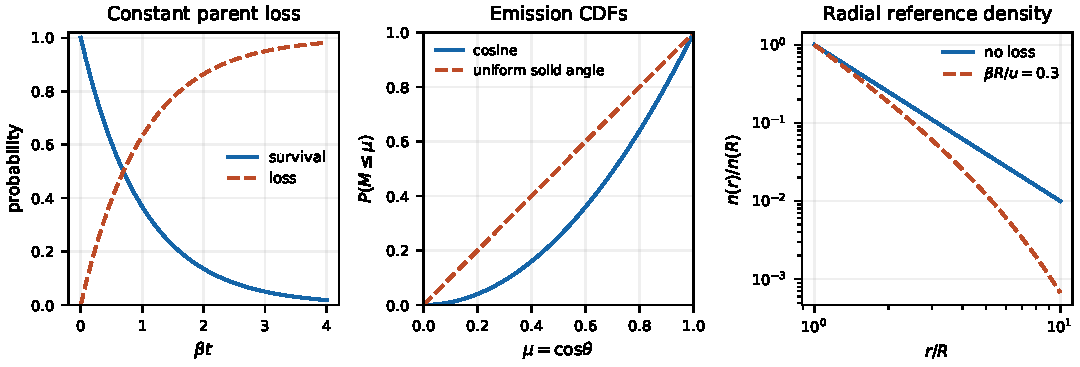
\includegraphics[width=\linewidth]{figures/kinetic_reference.pdf}
\caption{Independent analytical limits, not simulation results. Left: constant
first-order parent loss. Centre: outgoing cosine-law and uniform-solid-angle
CDFs in the normal-direction cosine. Right: steady spherical constant-speed
outflow, $n(r)/n(R)=(R/r)^2\exp[-\beta(r-R)/u]$, excluding gravity, collisions,
returning particles and distributed sources. These limits illustrate different
normalization and physical assumptions; they are not universal coma solutions.}
\label{fig:reference-limits}
\end{figure}

\section{Time step, mesh resolution and particle weight}
A common transport constraint for a global step is
\begin{equation}
\Delta t\leq \min_{s,b,d}
\frac{C_s h_{b,d}}{v_{\mathrm{char},s}},
\qquad 0<C_s\leq 1 ,
\end{equation}
with cell lengths $h_{b,d}$ in metres and speed in metres per second.
This is an application-selected characteristic-speed bound, not a guarantee
against the tail of a Maxwellian. Gyromotion, field variation, chemistry and
collision accuracy can impose stricter limits. Log actual minimum cells and
the final accepted step, not just the requested resolution.

For a constant physical source $Q_s$ and an expected $N_s$ numerical
injections per step, $W_s=Q_s\Delta t/N_s$ when all particles use one weight.
For a source with acceptance/rejection, local time steps or importance
sampling, derive the represented \emph{accepted} rate and its correction
instead of applying that expression blindly.
For local face transfer the represented crossing rate is $Wc/\Delta t$.
The opt-in resampling multiplicity is
\begin{equation}
\mu_{\rm face}=\frac{W_{\rm old}\Delta t_{\rm new}}
{W_{\rm new}\Delta t_{\rm old}} .
\end{equation}
The individual correction cancels only under the implemented policy of
holding that correction fixed. Continuation across MPI owners must finish
before sampling or generic splitting can duplicate an unfinished trajectory.

\section{Choosing a discretization for DSMC}
Resolve the shortest relevant density/temperature/flow scale and assess cell
size relative to mean free path. Separate transport and collision time errors.
For a dilute single-species estimate,
$\lambda\sim1/(\sqrt{2}n\sigma)$; mixtures and speed-dependent cross sections
require an appropriate collision integral. Refine where collisional and
surface gradients are strongest, then demonstrate convergence of the
actual observable. Increasing particles alone does not remove mesh bias.

Representative counts per collision cell must support the selected pair
algorithm. Sparse cells can have biased or noisy rates even when the total
particle population is large. A large sample window does not remedy a
systematic collision-cell or trajectory error.

\section{Sampling, stationarity and uncertainty}
Discard startup transients based on relaxation/transport times and observable
histories, not an unexplained iteration count. A sampling length in steps
corresponds to $N_{\rm sample}\Delta t$ only for a fixed global step.
Retain the actual physical accumulation interval for variable-step estimators.
Estimate uncertainty using independent realizations or block averages long
enough to expose autocorrelation. The familiar $N^{-1/2}$ statistical scaling
does not justify treating correlated stored samples as independent.

Separate three studies: mesh refinement at controlled statistics, timestep
refinement at controlled mesh, and particle/sample refinement at fixed
discretization. Include boundary-distance and external-data resolution studies
when those control the observable. Never fit a source with one numerical
error and interpret the compensation as a measured physical rate.

\section{Random streams and population control}
Record seed, rank/thread layout and stream policy. Reproducibility on the
same layout does not imply identical particles after repartitioning.
For a constant Poisson rate $\nu$, sample
$\tau=-\log(1-u)/\nu$ with the generator's declared endpoint convention.
Numerically \code{-log1p(-u)} resolves small $u$ well; replacing the draw by
\code{-log(u)} changes a fixed seeded path even though both have the same
continuous distribution.

Generic split/merge must preserve the moments required by the application,
and must specify what happens to opaque extension bytes. Conserving number,
momentum and scalar energy does not preserve all angular or higher moments.
Dust requires its own size-sensitive rules (Chapter~\ref{ch:dust}).
\source{src/pic/README.md; test/srcCoreUnitTests/README.md}

\chapter{Adaptive mesh, geometry and interpolation}\label{ch:mesh}
\section{Tree, blocks and dimensionality}
AMPS uses an adaptive tree with $2^D$ children per refined node in represented
dimension $D$. Leaves identify physical mesh blocks; blocks contain configured
cell and ghost-cell counts. Tree topology, allocated blocks, particle lists
and cell-associated fields are different objects with different ownership.
DIM1 radial geometry additionally requires spherical measures; it is not
equivalent to a Cartesian line with unit cross section.

For a radial spherical shell, the exact volume per steradian is
\begin{equation}
V_\Omega=\frac{r_R^3-r_L^3}{3}
=\frac{(r_R-r_L)(r_R^2+r_Rr_L+r_L^2)}{3}.
\end{equation}
The factored form avoids subtraction of nearly equal large powers. Use a
consistent volume centroid and surface measure in sampling, source and
transport operators. A visually plausible radial grid with Cartesian
normalization produces a physically incorrect density.

\section{Resolution functions and adaptation}
An application resolution function requests scales; the realized dyadic mesh
is what controls transport and resource use. A flyby or limb ray can require
refinement away from a surface. Refine the comparison region explicitly and
record actual cells intersecting each observation, rather than relying on
a small surface-cell size to resolve an entire trajectory.

Adaptation requires transfer policies for persistent state, sampled moments
and particle ownership. Coarsening must not simply average quantities whose
physical measure differs. Distinguish conservative extensive quantities from
primitive intensive state. A changed mesh invalidates cached stencils and
owner mappings. Verify generation changes and restored connectivity through
refine/coarsen cycles and mesh-file round trips.

\section{Interpolation contracts}
AMPS provides legacy pointer stencils and decomposition-independent row
stencils. A row identifies physical owner cells even if their blocks are not
allocated on the requesting rank. This is useful for exchanged fields and
distributed output; it does not make remote values locally accessible without
an exchange.

Constant fields should be reproduced exactly within rounding error. A linear
Cartesian field
$g=1.25+2x-3y+0.5z$ is an independent trilinear interpolation oracle.
At a coarse/fine interface, verify support, nonnegative weights, unit sum and
affine reproduction. A sum-to-one check alone cannot detect a geometrically
wrong stencil. Test every applicable face, edge and corner orientation,
boundary truncation, periodic wrapping and cache invalidation.

\section{Cut cells and internal boundaries}
A triangulated surface intersects cells and modifies accessible physical
volume. Surface interception and volume integration are distinct numerical
tasks. A mover can correctly hit a triangle while a cell-density normalization
still uses an incorrect accessible volume. Very small cut cells require a
defined normalization/time-step policy; do not silently replace their volumes
with a floor without changing and validating the model.

Independent geometry controls include a planar cut of known volume,
translated spheres, triangle areas/normals, tangent rays and convergence of
area/volume with geometric resolution. Mesh topology and triangle indexing
must survive reading, writing and reloading sparse external IDs.

\section{Distributed geometry and output}
Halo exchanges must transfer the correct fields for the current mesh and
sampling generation. Mesh serialization and restart traverse $2^D$ children,
not a hard-coded eight in lower dimensions. DIM1/DIM2 stored face caches
still need valid initialization if a persistent mesh format reads them.

Geometry-only Tecplot output does not validate physical field callbacks.
Whole-brick data output does not automatically clip an internal sphere.
Select the cut-cell-aware distributed writer when clipped boundary geometry
is required, and validate both geometry and data ordering.
\source{test/srcCoreMeshTests/README.md; test/srcCoreMPITests/README.md; src/README.md}

\chapter{Particle movers, forces and field solvers}\label{ch:movers}
\section{Neutral and charged characteristics}
For a neutral under a prescribed force,
$\dot{\boldsymbol x}=\boldsymbol v$ and
$\dot{\boldsymbol v}=\boldsymbol F/m$.
Gravity from a spherical body is
$-\mathcal GM\,\boldsymbol r/r^3$ outside its mass distribution, with
$\mathcal GM$ in $\mathrm{m^3\,s^{-2}}$. Nonspherical gravity requires a
separately defined mass model; a surface shape alone does not determine it.
Radiation pressure and gas drag are distinct accelerations with their own
size, velocity and geometry dependence.

Charged-particle trajectories satisfy
\begin{equation}
\dot{\boldsymbol v}=\frac{q}{m}
(\boldsymbol E+\boldsymbol v\times\boldsymbol B)+\boldsymbol a_{\rm other}.
\end{equation}
The relativistic equation advances momentum
$\boldsymbol p=\gamma m\boldsymbol v$ with
$\gamma=\sqrt{1+p^2/(m^2c^2)}$; replacing $m$ by a constant guessed
relativistic mass is generally incorrect. Validate gyrofrequency, phase,
parallel acceleration and drift against independent solutions.

\section{Selecting a mover}
The ordinary host dispatch is
\code{PIC::Mover::DispatchParticleMover(ptr, dt, node)}.
Legacy macro selection remains the default. Pointer selection requires its
compiled legacy-settings switch to be off and a valid
\code{PIC::Mover::SetUserDefinedParticleMover} callback installed before
advancing a particle. Boundary-specific or device bulk kernels can have
separate selection paths. The callback owns deletion/list insertion/migration
according to the configured mover contract.

The timestep must resolve the fastest relevant gyroperiod and field scale,
as well as cell crossings. Guiding-center motion assumes gyroaveraging is
valid: gyroradius and gyroperiod must be small relative to background scales.
Its drifts, mirror force and parallel electric force are not a valid fallback
at a magnetic null; the field-local API provides typed invalid-domain status.

\section{Electromagnetic PIC and ECSIM}
Self-consistent PIC deposits particle charge/current and solves fields rather
than reading a prescribed background. ECSIM is an energy-conserving
semi-implicit formulation in the supported configuration. Verify the actual
spatial operators, mass/moment assembly, boundary rows, solver residuals and
particle-field energy accounting. Stability of a semi-implicit method does
not remove resolution requirements for the phenomenon of interest.

For deposited shape weights $S_i$, require the intended partition of unity
and $\sum_i Q_i=q w$ for one particle. Current conservation additionally
requires a compatible discrete continuity equation, not just a correct total
charge. Manufactured field tests establish consistency of operators on the
tested meshes; they are not a blanket validation of every production plasma.

\section{Boundary events and complete trajectories}
Find the earliest physical boundary intersection within the remaining
trajectory interval. Reflect or absorb at that event, then process the
remaining time exactly once. A particle reaching a remote block must be
delivered to its owner even if its continuation marker is already zero.
Repeated reflection, tangency and starts on/inside a boundary need explicit
tolerance and ownership conventions.

Use independent straight-line, constant-acceleration, uniform-field gyro,
moving-plane and moving-sphere solutions as test oracles. Check phase-space
invariants, event time, list membership, endpoint and represented losses;
checking only final radius misses wrong velocity and duplicate ownership.
\source{src/pic/README.md; test/srcCoreUnitTests/README.md; src/test/tests/pic/ecsim_operators/README.md}

\chapter{Collisions and internal degrees of freedom}\label{ch:collisions}
\section{Binary collisions and the DSMC approximation}
DSMC separates molecular free flight from stochastic collisions over a short
physical interval \cite{bird1994}. Pair selection is local to a collision cell.
For species densities $n_a,n_b$, the physical cross-species rate per volume is
\begin{equation}
R_{ab}=n_a n_b\langle \sigma_{ab}(g)g\rangle,\qquad
g=|\boldsymbol v_a-\boldsymbol v_b|.
\end{equation}
For identical species the unordered-pair rate contains a factor $1/2$.
Finite populations require the appropriate pair-count correction; sampling
the same numerical particle twice is not a physical self collision.

Elastic scattering preserves pair momentum and relative kinetic energy.
Use the mass-weighted centre velocity and reduced mass:
\begin{equation}
\boldsymbol V=\frac{m_a\boldsymbol v_a+m_b\boldsymbol v_b}{m_a+m_b},
\qquad E_{\rm rel}=\tfrac12\frac{m_am_b}{m_a+m_b}g^2.
\end{equation}
An isotropic hard-sphere angular law and a VSS angular law have different
transport properties even when their total cross sections agree.

\section{Models, parameters and selection}
Hard-sphere (HS), variable-hard-sphere (VHS) and variable-soft-sphere (VSS)
selectors are tested in separate compiled profiles. HS uses a constant total
cross section. VHS introduces a speed dependence associated with the chosen
viscosity exponent; VSS additionally changes the scattering-angle
distribution. Read the generated reference-temperature, reference-cross-section
and exponent conventions together: copying an exponent between definitions
without its normalization changes the rate.

Use a collision database only within the declared temperature/energy range.
A missing species pair, an out-of-range law and a zero physical rate are
different states. The reusable comet collision database makes those
distinctions explicit. Record the pair law, units, source and valid range in
the run provenance rather than describing the model simply as collisions on.

\section{No-time-counter selection and unequal weights}
The NTC algorithm uses a majorant of $\sigma g$ and a rejection step.
The majorant, trial normalization and accepted-particle update probabilities
must describe the same weighted population. A diagnostic trial count by
itself is not the physical collision count.

In the implemented general correction-aware NTC path, physical carrier
$q_i=W_s c_i$ determines weighted selection. Cross-species trials use
\begin{equation}
N_{\rm trial}=\frac{(\sum_iq_i)(\sum_jq_j)
(\sigma g)_{\max}\Delta t_{\max}}{q_{\min}V}.
\end{equation}
Selected particles are updated with the prescribed $q_{\min}/q_i$ and
local-timestep factors. Same-species self draws are discarded, not repeatedly
redrawn with a different pair law. The simplified kernel is not a substitute:
it explicitly rejects the unsupported correction-on configuration.

Dust is excluded before gas-species prefix sums are constructed. Otherwise a
steep grain weight distribution can perturb gas pair selection even if no
grain is ultimately collided. Reusable thread-local species buckets reduce
allocation overhead without changing the intended traversal order.

\section{Rotational and vibrational energy}
For $f_{\rm rot}$ classical quadratic rotational degrees of freedom, equilibrium
mean energy is $f_{\rm rot}k_BT/2$. Larsen--Borgnakke redistribution samples a
microcanonical energy partition when the selected relaxation event occurs.
The relaxation number $Z_{\rm rot}$ controls an event probability, not an
energy multiplier: the maintained $Z=2$ and $Z=10$ profiles independently
check probabilities $1/2$ and $1/10$.

For an ideal harmonic vibrational mode with characteristic temperature
$\Theta_v$, the thermal energy above its ground state is
\begin{equation}
\langle E_v\rangle=\frac{k_B\Theta_v}{\exp(\Theta_v/T)-1}.
\end{equation}
Use the production model's level convention and degeneracies. Equilibrium
sampling, rotational relaxation, vibration--translation and vibration--vibration
rates are separate capabilities; a rotational test does not establish all of
them. Chemical formation energy must not be counted again as an internal
relaxation source.

\section{Independent validation}
The core suites compare rates with analytic HS moments and independent
Maxwell relative-speed quadrature for VHS. VSS checks angular moments as well
as elastic invariants. Native particles in a 3-D AMR cell exercise actual
collision and rotational-relaxation routines. Assess statistical error on
accepted physical rates, relaxation times and equilibrium moments, and
separately monitor conservation. A conservation-only test can pass a routine
that performs no collisions at all.

\scope{The documented tests cover bounded selectors and profile combinations.
They do not qualify every unequal-weight collision law, every species-dependent
relaxation model or all VT/VV processes. Consult the test receipt and profile.}
\source{src/pic/README.md; test/srcCoreUnitTests/README.md; src/models/cometary_physics/README.md}

\chapter{Photochemistry and other reactions}\label{ch:chemistry}
\section{Rates, channels and parent survival}
For a constant first-order loss frequency $\beta$ in $\mathrm{s^{-1}}$,
\begin{equation}
P_{\rm survive}(\Delta t)=e^{-\beta\Delta t},\qquad
P_{\rm loss}=1-e^{-\beta\Delta t}.
\end{equation}
Compute small loss probabilities accurately, for example with
\code{-expm1(-beta*dt)}. For time-varying illumination or rates, the exponent
is $-\int\beta(t)\,dt$ along the actual trajectory. A constant-rate fixture
cannot validate occultation crossings or a nonuniform radiation field.

For competing constant channels $\beta_j$, sample the event time from
$\sum_j\beta_j$ and channel $j$ with probability
$\beta_j/\sum_k\beta_k$. An already committed event must not be repeated
by another driver. Multiplicity belongs to stoichiometry: a channel producing
two H atoms is not equivalent to a channel producing one H atom at twice its
weight unless the chosen estimator explicitly proves that equivalence.

\section{Daughters and event energetics}
A parent-loss-only application deletes or changes the represented parent
without allocating daughter particles. It must explicitly disclose that
product transport and product conservation are outside its particle model.
A daughter-producing application additionally owns species identity, product
weights, insertion cells and velocity/internal-energy laws.

For a two-product channel with available translational energy $E_{\rm ex}$,
zero centre-of-mass momentum gives opposite momenta of magnitude
\begin{equation}
p_*=\sqrt{2\mu E_{\rm ex}},\qquad
\mu=\frac{m_1m_2}{m_1+m_2}.
\end{equation}
Transform products into the parent's inertial frame. Multibody products,
electrons, ionization thresholds and internal excitation require their own
partition laws; do not apply this two-body formula indiscriminately.
Reaction tables must distinguish photon energy, threshold, recoil energy
and energy already assigned to internal modes.

\section{Charge exchange and electron impact}
For incident particles in a background population, a typical charge-exchange
frequency is $n_{\rm bg}\langle\sigma g\rangle$. Resonant exchange can swap
charge labels while retaining the physical neutral/ion velocity roles; it
is not automatically removal of the neutral with no product. Electron-impact
rates require the correct electron distribution, threshold and cross-section
or rate fit. Units of $\mathrm{m^3\,s^{-1}}$ and $\mathrm{cm^3\,s^{-1}}$
must not be mixed.

The T6 native reaction owner checks optional charge-exchange and Burger
electron-impact archives, branch identities and thresholds. That owner does
not authorize those processes in an application whose input schema rejects
plasma reactions. Rates inferred at a heliocentric distance or solar state
must be converted once, with the selected scaling and provenance recorded.

\section{Networks, stiffness and weighted estimators}
The reusable reaction network expresses stoichiometry, channel rates and
product multiplicities independently of a comet geometry.
The chemical solver has separate analytic decay/kinetics, positivity and
stiff-system tests. A deterministic abundance solver and stochastic
particle chemistry solve related equations with different numerical errors.
Neither is an independent reference if expected values are generated by the
same implementation being graded.

The generic comet application supports population policies, correction windows,
daughter packets, channel importance sampling and optional total-reaction
forcing. These are unbiased-estimator requirements, not extra chemical
channels. Preserve signed/residual estimator state through adaptation,
migration and restart. Changing a proposal law requires an explicit physical-
to-proposal weight ratio and independent rate/product-budget tests.

\section{Transactional production callbacks}
The ordinary photolysis callback remains available. An optional batched
interface consists of begin, eligibility, batch-limit, reaction-processor
and end-pass callbacks. All five must be installed together.
Each event commits completely or leaves a deferred parent unchanged;
new daughters are not eligible to be processed again in the same parent pass.
The pre-exchange callback can create particle-buffer headroom before receive
allocation. A partial callback set or an unsupported hybrid mode is rejected.

\section{The Enceladus parent-loss scope}
The maintained schema-2 example transports neutral H2O and CO2. The selected
Burger water photo channels remove H2O parents; products are discarded.
CO2 is transport-only in this receipt. No plasma background or daughter
species may be inferred from the compiled species list. The exact ledger is
\begin{equation}
N_{\rm injected}=N_{\rm photo}+N_{\rm surface}
+N_{\rm escape}+N_{\rm resident}
\end{equation}
per primary species, in the represented-particle convention of the run.
\source{srcHartley2/CHEMISTRY.md; srcEnceladus/test/README.md; src/models/chemical_solver/README.md}

\chapter{Dust grains and grain populations}\label{ch:dust}
\section{Size is a physical state}
Dust is not a gas species with a larger fixed mass. Radius, material density,
charge, velocity and any optical/material properties control its dynamics.
For an ideal sphere of radius $a$ and density $\rho_d$,
\begin{equation}
m_d=\frac{4\pi}{3}\rho_da^3,\qquad
\phi=\frac{q_d}{4\pi\epsilon_0a},\qquad
\boldsymbol a_L=\frac{q_d}{m_d}
(\boldsymbol E+\boldsymbol v\times\boldsymbol B).
\end{equation}
The potential relation assumes an isolated spherical conductor. Shielding,
nonspherical grains and material effects require different closures.
The Lorentz term includes neither gas drag, gravity nor radiation pressure.

\section{Size distributions and importance weights}
For a number distribution $d\dot N/da=Ca^{-p}$ on
$[a_{\min},a_{\max}]$, total number and mass rates are different integrals:
\begin{align}
\dot N&=C\int a^{-p}\,da,\\
\dot M&=\frac{4\pi\rho_dC}{3}\int a^{3-p}\,da .
\end{align}
The logarithmic limits $p=1$ and $p=4$ must be evaluated with their proper
logarithms. A specified dust mass source does not determine a numerical
particle weight until the size proposal and material density are given.
For proposal density $g(a)$, an event's represented contribution contains
the physical density divided by $g(a)$. This correction is independent of
generic population splitting/merging.

The PIC-coupled dust model requires positive individual weight corrections.
Logarithmic radius bins are half-open, with the global upper endpoint owned
by the final bin. A steep number distribution can coexist with most of the
injected mass in the largest grains. The in-coma size distribution additionally
depends on size-dependent speed and survival; it need not reproduce the
source distribution.

\section{Charging and forces}
Charging integrates currents appropriate to the declared plasma/illumination
model. Validate equilibrium roots and transient convergence across multiple
radii, including the sign convention for collection and emission currents.
A floating potential can be small while charge-to-mass acceleration is large.
If plasma inputs are absent, an explicit neutral/uncharged model is required;
zero-filled background data are not a physically justified charging solution.

Gas drag, radiation pressure, gravity and Lorentz forces have distinct
validity regimes. Couple each force to the same grain state and frame.
Radiation/optical interpolation tables need wavelength, radius, refractive-
index convention and out-of-range policy. A Mie table lookup test is not
validation of an entire dust tail.

\section{Dust-specific split and merge}
The dependency-light dust API groups particles by log radius and requires the
same native owner cell, compiled species and size group. Current merging
additionally requires exactly equal intrinsic radius, mass and charge.
Same-bin membership alone is insufficient: two radii can have different
charging and drag physics even if their difference looks small numerically.

Splitting clones one grain into $n$ representatives with weights $w/n$.
The supported merge maps at least three compatible particles to two:
total weight $W$, weighted mean velocity $\boldsymbol u$, and velocities
$\boldsymbol u\pm d\boldsymbol e_j$, each with weight $W/2$, where
$d^2$ is the weighted velocity variance. It conserves represented number,
mass, charge, momentum and scalar kinetic energy. It does not generally
preserve the pressure tensor, higher moments or mean speed. The API can
reject a requested sampled-speed constraint transactionally.

\scope{The dust split/merge physical kernel is implemented and tested.
A general production PIC-list adapter is not supplied by that algebraic
PASS. Generic gas split/merge must not be used to erase radius-dependent
physics.}

\section{Spherical injection and its ledger}
The production sphere injector chooses surface position relative to the
actual centre, applies native ownership and local-time acceptance, creates
the record and dispatches the selected mover. A signed residual mass reservoir
accounts for finite particle granularity. A negative residual is not negative
physical grain mass; it records that an event has advanced a fractional budget.
The native fixture checks this ledger over two intervals and verifies that
gas NTC leaves steep-weight grain records unchanged.
\source{src/models/dust/README.md; test/srcModelDustTest/README.md; test/srcModelDustInjectionTest/README.md}

\chapter{Surfaces, arbitrary shapes and source boundaries}\label{ch:surfaces}
\section{Geometry is separate from surface physics}
Supported application geometries include analytic spherical boundaries and
triangulated surfaces with cut-cell operations. Terrain-derived lunar meshes
and comet shape models add data requirements. A valid triangle mesh does not
specify temperature, composition, adsorption, sputtering yield or gravity.
Those are explicit physical closures.

Let $\boldsymbol n$ point from the solid into the gas. An incident particle
has $(\boldsymbol v-\boldsymbol u_{\rm wall})\cdot\boldsymbol n<0$.
Always state the surface-normal and wall-velocity conventions. For specular
reflection,
\begin{equation}
\boldsymbol v'=\boldsymbol v-
2[(\boldsymbol v-\boldsymbol u_{\rm wall})\cdot\boldsymbol n]\boldsymbol n .
\end{equation}
The invariant is kinetic energy in the local wall frame, not necessarily in
the inertial frame. Moving walls can exchange physical work with particles.

\section{Diffuse emission and accommodation}
Fully diffuse thermal emission from a stationary surface at temperature $T$
uses the outgoing flux distribution. With thermal tangential components,
the positive normal component obeys
\begin{equation}
p(v_n)=\frac{m}{k_BT}v_n e^{-mv_n^2/(2k_BT)},\qquad v_n>0.
\end{equation}
Thus $v_n=\sqrt{-2k_BT\log(1-u)/m}$. Sampling the positive half of an ordinary
Maxwellian is not the same boundary flux law.
For Knudsen/cosine angular emission over the hemisphere,
$p(\mu)=2\mu$, $0\leq\mu\leq1$, so $\mu=\sqrt u$; uniform solid angle
instead has uniform $\mu$. Isotropic surface position is another independent
distribution. Use the selected law explicitly.

Accommodation, sticking, adsorption and desorption are separate probabilities
or fluxes. Preserve a surface inventory balance,
\begin{equation}
N_{\rm surf}^{n+1}=N_{\rm surf}^{n}
+N_{\rm ads}-N_{\rm des}+N_{\rm other},
\end{equation}
with all terms using the same element area, time interval, species and
represented weight. Emptying a flux buffer must not empty the physical
surface reservoir.

\section{Exosphere source processes}
Applications can combine thermal desorption, photon-stimulated desorption,
impact vaporization, sputtering, vertical or user-defined emission.
Each has its own yield, energy/angular law, surface depletion and illumination
dependence. A uniform sputtering rate fixture does not validate a
plasma-dependent yield table. The native spherical exosphere owner compiles
and exercises five bounded source modes with independent rate/inventory
ledgers; external/background injection is a domain-boundary process with a
different contract.

\section{Importing an arbitrary shape}
Before using a NASTRAN/triangle shape:
\begin{enumerate}
\item Declare coordinate units, body origin, orientation, epoch and external
ID convention. Scale exactly once into the application frame.
\item Reject malformed connectivity, zero-area facets and invalid IDs.
Inspect normals and winding. A closed body needs a consistent inside/outside
definition; an open sheet needs an explicitly different physical treatment.
\item Verify bounds, known lengths, signed/enclosed volume where meaningful
and surface area under controlled refinement.
\item Check rays, tangencies, shared edges, concavities and translated copies.
Round-trip the actual format without assuming dense consecutive node IDs.
\item Resolve local geometric features with the transport/cut-cell mesh and
establish area/volume and observable convergence.
\end{enumerate}
Generic I/O tests use synthetic sparse IDs and known geometry. They do not
certify an arbitrary production shape for watertightness, self-intersection,
small features or surface-source mapping. Large concave shape integrations
can be costly during initialization even before the first particle step.

\section{Source positions and normalization}
For a uniform triangle, two uniforms can be transformed to barycentric
weights with $\sqrt{u}$; choosing two unconstrained barycentric coordinates
biases the area. Choose triangles proportional to integrated physical
emission, not by triangle count unless every element has equal rate.
For a source shape $f_i\geq0$ used with total $Q$,
$Q_i=Q f_i/\sum_j f_j$; an absolute source file already supplies $Q_i$.
Reject a contradictory additional total in absolute mode.

Enceladus uses projected surface jets/stripes rather than adopting all their
unprojected empirical fitting coordinates as physical launch points.
Moon terrain, spherical exosphere and arbitrary comet surfaces have separate
source/thermal adapters. An unchanged source file is part of comparison
provenance, especially if rates were fitted to the same observations.
\source{test/srcCoreExosphereTests/README.md; test/srcCoreMeshTests/README.md; srcEnceladus/SOURCE_DISTRIBUTION_FILE.md}

\chapter{Planetary, satellite and comet applications}\label{ch:planetary}
\section{A common kinetic engine, different physical targets}
Planetary applications choose their own body shape, rotation, gravity,
illumination, surface inventories, plasma/radiation fields and observation
operators. A species list or successful mesh initialization is not a complete
physical model. Record the target, epoch, frame, source law and loss/network
scope with every run. Use ephemerides and orientation consistently in
injection, acceleration, surface interception and synthetic observations.

\section{The Moon: exosphere, terrain and observation geometry}
\path{srcMoon} combines spherical or terrain-based surface geometry with
target-specific exosphere processes and diagnostics. Its generic runtime
block is selected with \code{-input FILE}; omission preserves the historical
analytic-sphere regression. The terrain path requires declared LOLA products,
labels, resolution and output paths. Do not replace unavailable topography
with a sphere without recording a different physical case.

Spatial targets distinguish the near-surface, far-field, terminator and polar
regions. Quick, regression and full science receipts are different numerical
campaigns. A completed coarse wiring run must retain its M1
SKIPPED/NOT QUALIFIED designation when convergence criteria were not exercised.
The lunar unit/integration runners cover geometry, source/thermal state,
environment timing and bounded products; inspect their actual per-case status.
Na tail and limb observations additionally require instrument geometry,
velocity-dependent radiation, line-of-sight weighting and the declared
exposure average.
\source{srcMoon/README.md; srcMoon/test/README.md; srcMoon/examples/README.md}

\section{Enceladus: sources, parent loss and Cassini comparisons}
\path{srcEnceladus} separates a fitted-source exporter from the forward kinetic
application. The currently implemented distribution identifier is
\code{tenishev2014_hybrid_8}: eight point jets and seven stripe components.
Stripe vertices are projected vertically onto the declared 252100-m reference
sphere. The separate source file states geometry, kinematics, frame and
whether strengths are absolute rates or a normalized shape.

Equal-strength E3/E5 receipts exist to start and exercise the forward code.
They are not a recovered individual-source fit. The E3/E5 mass-44
normalizations are apparent CO2 and carry a documented impact-fragmentation
bracket; they must not be reported as unqualified physical CO2 production.
The schema-2 run transports neutral H2O/CO2 with selected H2O photolytic
parent loss only, no daughter particles and no plasma.

Observation requests select INMS density/count products and supported UVIS
occultations. Density, detector count rate and occultation transmission are
different operators. Only compare like quantities with compatible response,
units, frame and epoch. A trajectory outside the mesh has no local density;
do not interpolate across that gap or label it zero. Resolve closest approach
with actual flyby cells, and plot sampling uncertainty and data availability.
\source{srcEnceladus/SOURCE_DISTRIBUTION_FILE.md; srcEnceladus/test/README.md}

\section{Comets: radial and shape-based gas/dust models}
\path{srcHartley2} retains its historical name but contains a generic comet
layer with a DIM1 spherical radial backend, legacy DIM3 shape application,
configurable chemistry/collisions, internal energy, cooling and brightness.
DIM2 axisymmetric execution is reserved rather than implemented. I3 uses
\path{input/i3.conf} for compiled capabilities and \path{input/i3.in} plus
\code{-case N} for physical cases. Halley and Hartley decks use their
documented workflows; do not assume every alias stages the shared parser
identically.

The radial backend retains three-dimensional velocity/trajectory geometry
while exploiting spherical symmetry for storage and sampling. It cannot
represent an arbitrary asymmetric jet or shadowed nonspherical coma.
For those cases use the appropriate DIM3 adapter with a qualified surface,
thermal map and gravity model. Nucleus production and escaping/net production
can differ because of returning particles; state which quantity is fitted.

The separate collisionless reference supplies a far-coma column correction
for selected I3 post-processing. It is not an extension of the DSMC domain.
Its columns, normalization, assumptions and missing radiation-pressure effects
are documented independently. Comparison tables imported from COMET1D are
historical evidence, not new runs of this checkout.
\source{srcHartley2/README.md; srcHartley2/COLLISIONLESS_REFERENCE.md; srcHartley2/i3/COMPARISON.md}

\section{Planetary energetic particles}
\path{srcEarth} includes backward-characteristic cutoff/access and
instantaneous spectrum products using declared static/quasi-static field
snapshots. A backward access calculation and a forward Monte Carlo density
calculation are different estimators. Field, spectrum, detector response and
observer epoch must form one accepted configuration with consistent units.
Classify unresolved/trapped/escaped characteristics explicitly; an unfinished
trajectory must not silently count as excluded flux.

The coupled Step-10/11 contracts produce content-identified snapshots and
product manifests. Their portable analytic/replay tests do not qualify
all external-data or live SWMF release matrices. Magnetic-only instantaneous
results do not imply electric acceleration or long-duration validity across
changing fields. Other planetary application directories require their own
input/data and acceptance review before reuse.
\source{srcEarth/README.md}

\chapter{Heliospheric and energetic-particle physics}\label{ch:helio}
\section{Field-line and three-dimensional formulations}
\path{srcSEP} transports particles along magnetic field lines embedded in
three-dimensional space and contains particle--Alfv\'en-wave coupling.
\path{srcSEP3D} supplies three-dimensional transport and background adapters.
They share physical libraries and input vocabulary where supported, but a
key accepted by one application need not be meaningful in the other.
The schema table marks ownership and unsupported combinations.

The isotropic Parker transport equation, in a common convention, is
\begin{equation}
\frac{\partial f}{\partial t}
=\nabla\cdot(\boldsymbol\kappa\nabla f)
-(\boldsymbol U+\boldsymbol v_d)\cdot\nabla f
+\frac{\nabla\cdot\boldsymbol U}{3}\,p\frac{\partial f}{\partial p}+Q.
\end{equation}
Here $f$ is phase-space density and $p$ momentum magnitude. Flux and
differential-energy spectra include additional Jacobians; a power index for
$f(p)$ is not automatically an index for $dN/dE$.
Focused transport additionally resolves pitch angle
$\mu=\boldsymbol v\cdot\boldsymbol b/v$, streaming/focusing and
pitch-angle diffusion. A diffusion approximation is not valid merely
because a mean free path parameter was supplied.

\section{Mean free path, diffusion and turbulence}
For suitable gyrotropic scattering,
\begin{equation}
\kappa_\parallel=\frac{v^2}{8}\int_{-1}^{1}
\frac{(1-\mu^2)^2}{D_{\mu\mu}}\,d\mu,\qquad
\lambda_\parallel=\frac{3\kappa_\parallel}{v}.
\end{equation}
Convergence near $D_{\mu\mu}=0$, resonance gaps and end points requires
an explicit model and quadrature policy. Perpendicular diffusion, field-line
wandering and deterministic drifts are different operators. Check
normalization, stochastic-calculus convention and any drift correction
against the actual stochastic differential equation.

The SEP tree includes integrated and wave-number-resolved turbulence,
advection/cascade and particle-wave terms. Their conservation and
normalization require matching wave energy, resonance convention and particle
weights. An uncoupled prescribed-turbulence test does not validate feedback.
The older detailed derivations retained in this directory are supplementary
reading; current public model contracts and test receipts determine support.

\section{Background providers and physical state}
An analytic Parker background, a PFSS/coronal ambient, a reduced front and
a full spatial CME have different capabilities. Record epoch, frame,
units, generation and validity interval for all sampled fields. Interpolation
must not silently substitute quiet ambient after a rejected shock solution.
Background advancement must not depend on particle allocation or source
planning when the selected background contract is particle-independent.

A reduced-front provider supplies the prescribed geometry, undisturbed
ambient reference and front-local immediate Rankine--Hugoniot limits.
It does not own a spatial sheath/ejecta volume. A geometric arrival is not
necessarily an accepted fast-shock arrival. Diagnostics must retain normal
speed, upstream-relative inflow, fast Mach number, obliquity, compression
and admissibility rather than imposing a compression floor.

\section{CME implementation and qualification boundary}
Shared coronal, SWCME, full-volume and reduced-front libraries have separate
software registries. Full-volume BG3D-4/G1 remains unqualified at this edition.
The selected resumed analytical lateral-material development retains the
3-D ambient, a field-threaded material contact and 1200-s startup corotation
transition. Bounded transport/mesh/CT/contact/Cauchy kernels are tested;
they do not constitute a production MHD runtime or a qualified regional map.

For a regular material map $\boldsymbol X(\boldsymbol a,t)$,
$F=\partial\boldsymbol X/\partial\boldsymbol a$, $J=\det F>0$, the adiabatic
Cauchy relations are
\begin{equation}
\rho=\rho_0/J,\qquad
\boldsymbol B=F\boldsymbol B_0/J,\qquad p=p_0J^{-\gamma}.
\end{equation}
They preserve material mass and flux for a compatible map; they do not select
that map, supply shock matching, or close force/heating/work budgets.
An isothermal expanding ambient needs explicit thermal work/heating beyond
the adiabatic subset.

The application can deliberately reject a source/provider even when its
library exists. In particular, current srcSEP3D documentation rejects the
unreleased SWCME runtime selection while preserving those decks as typed
negative fixtures. The reduced-front source has a bounded constant-weight
mode; log-uniform momentum importance remains reserved until its individual
weight correction is implemented and qualified. Read the application
capability check before selecting a historical example.
\source{srcSEP/README.md; srcSEP3D/README.md; src/models/sep_corona_swcme/README_CROSS_RAY.md}

\chapter{SWMF and external background coupling}\label{ch:coupling}
\section{Component lifecycle}
SWMF builds model libraries into one framework executable. AMPS supplies PT
(particle tracker) and PC (particle-in-cell) wrappers in \path{srcInterface}.
The control module owns component registration, processor layout, sessions,
execution/coupling schedules and framework restart requests.
An AMPS standalone executable does not pass through the same outer driver.

The wrapper actions include VERSION, MPI, READ, CHECK, STDOUT, FILEOUT and
GRID, followed by session initialization, run, restart and finalize methods.
READ can occur multiple times before CHECK. Fields and mesh descriptions
must not be published before their initialization stage. The current AMPS
wrappers contain partly stubbed checking/output-routing actions; this manual
does not promote them to a validated full implementation.

\section{Communicators and processor layout}
Use the communicator supplied by the framework. The Fortran handle is
converted with \code{MPI_Comm_f2c}; collective calls must involve exactly
that component's participating ranks. Overlapping component processor sets
execute sequentially on shared ranks. Disjoint sets permit concurrent
evolution, subject to data dependencies. Thread support and actual affinity
must be checked separately from processor counts.

A schematic two-component layout, in a SWMF \path{PARAM.in}, is:
\begin{lstlisting}
#COMPONENTMAP
GM  0  1  1
PT  2  3  1
\end{lstlisting}
It requires four ranks and compatible compiled components. This is a layout
fragment, not a complete runnable physical case.

\section{Parameter ownership and schedules}
SWMF compile-time model selection uses its own \code{Config.pl -v=...}.
Its \code{#BEGIN_COMP PT} block carries component parameters; standalone
AMPS generic runtime input is a different grammar.
Always validate against the actual SWMF \path{PARAM.XML} and component XML:
some historical prose examples reverse positional arguments.
For example, a one-way physical-time cadence uses:
\begin{lstlisting}
#COUPLE1
GM          NameSource
PT          NameTarget
-1          DnCouple
10.0        DtCouple
\end{lstlisting}
This is a 10-s schedule, not a physical justification for that interval.
Time-accurate components must respect supplied synchronization limits.
Tight coupling additionally requires a supported master/slave timestep
contract. Permitting a component to step past a coupling epoch changes
temporal accuracy and must be declared.

Three clocks matter: iterations since process start, accumulated steps
including restart history, and physical simulation time. Returning a limit
to the scheduler without advancing a physical state to that epoch is not
evidence of synchronization. Test this explicitly for nonintegral ratios of
the AMPS step to coupling interval and for first-data readiness.

\section{Exchange contracts}
Each exchanged quantity needs a species/fluid mapping, units, frame,
location (cell centre, corner, face or field-line vertex), timestamp and
validity. Transform vectors, velocities and electric fields with the
correct frame convention; rotating-frame velocity is not just a rotation
of an inertial vector. Keep magnetic interpolation compatible with any
required divergence or flux constraint.

Exchange a coherent state generation rather than mixing fresh density with
old velocity. Verify owner and received-ghost values independently. A
successful send count is not proof of correct physical data. Negative tests
should reject missing variables, nonfinite values, stale epochs, mismatched
layout and unsupported fluid counts before particles consume them.

\section{File providers, SPICE and empirical models}
Offline backgrounds need a versioned file format, dimensional identities,
frame/epoch and explicit missing-domain policy. CDF/Kameleon, BATSRUS/BATL,
ARMS, CCMC and SWMF are separate optional interfaces with different fixtures.
Finding a library on disk does not qualify its adapter.
SPICE supplies geometry, not plasma. Record exact kernel versions, load order,
coverage and target/frame/aberration choices. Kernel readiness requires real
state/orientation queries for the requested epoch.

\section{Coupled testing and isolation}
SWMF's legacy test Makefile serializes its top-level recipes and suppresses
some command failures while retaining \path{.diff} artifacts. A wrapper runner
must inspect expected outputs and classify missing evidence as ERROR.
Never concurrently reconfigure the same SWMF/AMPS build tree for independent
tests. Run isolated runtime cases from frozen executables after serialized
configuration/build, keeping each result separate before aggregation.

The AMPS global SWMF provider case remains SKIP without an independently
registered exchange fixture. Synthetic ABI or replay tests are valuable but
do not replace a live component-communicator and exchanged-field test.
\source{srcInterface/PT_wrapper.f90; srcInterface/PC_wrapper.f90; srcInterface/amps2swmf.cpp}

\chapter{Sampling, output, observations and restart}\label{ch:output}
\section{Data lifetime and normalization}
Accumulate raw represented moments into the collecting sample, then publish
a completed window. Normalize once using the actual volume, exposure/time
and sample measure. The completed buffer must remain immutable while output
reads it. Clearing or swapping a buffer is a lifecycle operation, not a
physical evolution of persistent background state.

For weighted velocity moments, temperature uses the bulk-subtracted tensor,
not mean speed squared. Cells with zero weight have undefined bulk moments;
write a defined empty/validity policy rather than a fabricated physical value.
Use physical cut-cell volumes where required. Distinguish number density
($\mathrm{m^{-3}}$), mass density ($\mathrm{kg\,m^{-3}}$), surface flux
($\mathrm{m^{-2}s^{-1}}$) and integrated column ($\mathrm{m^{-2}}$).

\section{Application-defined node data and Tecplot}
Register static/sampled storage and output callbacks before layout freezing.
Output consists of variable names, interpolation and value printing in the
same order. Interpolation can touch temporary nodes that have no associated
AMR block: callbacks must not assume every printed node is owner-local.
Populate owner state and exchange required ghosts before printing.

\code{outputMeshTECPLOT} is geometry-only.
\code{outputMeshDataTECPLOT} and
\code{OutputDistributedDataTECPLOT} have different boundary/parallel traversal
contracts. A registered sphere does not automatically clip whole output
bricks. Use the writer appropriate to the geometric product and verify
variable order, units, finite records and owner/ghost agreement.

Full-volume ASCII output can dominate disk and runtime. Prefer a declared
trajectory/ray product when it supplies the observable, retaining the same
completed sampling window. Suppressing a visualization dump must not suppress
physical accumulation or its conservation receipt.

\section{Synthetic observations}
For an optically thin emissivity with effective fluorescence rate $g$,
brightness involves $\int n g\,ds$ with the chosen radiance convention and
solid-angle conversion. Do not replace a velocity-dependent $g$ with a
constant unless that approximation is part of the model. Occultation
transmission instead uses optical depth
$\tau_\lambda=\int n\sigma_\lambda\,ds$, with $I/I_0=e^{-\tau_\lambda}$
in the simple absorption limit. Detector count rates additionally require
response, binning, viewing direction and background treatment.

Evaluate spacecraft density at its actual ephemeris and epoch. Map all
comparison inputs to the same frame. Distinguish missing observations,
out-of-domain model points and physical zeros. Record source-fit provenance:
agreement with data used to fit a source is not independent validation.

\section{Persistent formats and restart identity}
Particle and data-file formats carry explicit kind/layout identities,
checksums and compatibility policy. Atomic publication avoids accepting
half-written output; it does not make an incompatible layout valid.
The global-weight particle restart layout remains revision 2;
local-weight restart has a separate revision-3 identity including block data.
Unversioned local-weight payloads are rejected.

Restart must preserve particles, weights, relevant time/RNG state, associated
application data and any residual chemical/source estimators. An empty cell
or block can still own physical state and must not be dropped solely because
it has no particles. After local block-state restoration, publish owner
values to ghosts before another face transfer.
Application-owned structured bytes need a semantic layout fingerprint:
an unchanged byte count alone does not identify a reaction-product ordering.

\section{Continuation and archive practice}
Verify both uninterrupted and split/restarted evolution with independent
budgets and selected observables. A same-binary file round trip proves less
than cross-decomposition continuation. A particle checksum alone does not
test sample buffers, surface inventories or chemistry residual state.
Do not interpret restart as a portable scientific interchange format.

Archive the exact executable hash, compile/runtime/source receipts, external
data hashes, seed/layout, units/frames, sampling intervals and process command.
Keep generated runs apart from maintained numerical reference fixtures.
Reference updates require scientific review; a new output is never its own
independent expected solution.
\source{src/README.md; src/pic/PERSISTENT_FORMATS.md; src/test/tests/pic/persistence/README.md}

\chapter{Verification, application tests and nightly reporting}\label{ch:tests}
\section{What the global procedure does}
\path{src/test/run_tests.py} selects exact suites/cases from a manifest, resolves
machine tools and prerequisites, runs individual owners and reconciles their
typed results. Core and registered application streams share one report.
The registry owns \emph{what may run}; individual adapters own their mechanics
and assertions; the component inventory owns the remaining coverage gaps.
An installed optional tool is not evidence that its scientific interface works.

Tests form several layers: dependency-light equations/algorithms, configured
native PIC applications, MPI ownership/halo/migration, application startup and
evolving end-to-end cases, portability/backend checks and expensive scientific
qualification. Select the layer required by the change. A parser/startup PASS
cannot replace an evolving simulation, and a regression reference cannot
replace a convergence or observational test.

The separately generated Makefile application regressions are documented in
Chapter~\ref{ch:application-regression} and individually cataloged in
Appendix~\ref{ch:legacy-catalog}. The 100 generated legacy owners are separate
from the modern 55-suite registry. Neither the global application's bounded
replacement tests nor the 13-directory legacy governance audit implicitly
executes every Table-controlled regression.

\section{Required machine configuration}
Every global invocation, including listing and coverage, requires
\code{--config}. Profiles live under \path{test/qualification-machine}, outside
the production source tree. Start from \path{template.json}; the checked-in
\path{passion.json} is one host's actual choices, not a universal default.
The profile records tools as argv vectors, output/work/data paths, MPI
launcher/rank flag, resource limits and optional capabilities.

Use a base profile and a small site/path overlay instead of editing runners:
\begin{lstlisting}
python3 -B src/test/run_tests.py \
  --config test/qualification-machine/passion.json \
  --config /path/to/local-overlay.json --campaign smoke
\end{lstlisting}
The second path is a placeholder the operator must provide.
Do not label unavailable SPICE, MPI, GPU, kernel or observation data as
available just to remove a SKIP. Set work/output paths to writable storage
with sufficient memory and quota. Distinguish compiler argv from shell text.

\section{Short, full and core-only commands}
All following commands run from the AMPS root. Use a new output directory
for each campaign.
\begin{lstlisting}
PROFILE=test/qualification-machine/passion.json

# Discover exact cases, grouped by stream.
python3 -B src/test/run_tests.py --config "$PROFILE" --list

# Fast control/library smoke campaign.
python3 -B src/test/run_tests.py --config "$PROFILE" \
  --campaign smoke --output-dir test_output/manual-smoke

# Every registered CORE owner; exclude application streams.
python3 -B src/test/run_tests.py --config "$PROFILE" \
  --match 'CORE-*' --jobs 8 --build-jobs 16 \
  --output-dir test_output/manual-core

# All routine registered streams.
python3 -B src/test/run_tests.py --config "$PROFILE" \
  --all --streams 3 --jobs 2 \
  --output-dir test_output/manual-all

# Explicit expensive/portability/distributed/qualification union.
python3 -B src/test/run_tests.py --config "$PROFILE" \
  --full-validation --streams 3 --jobs 2 --build-jobs 16 \
  --output-dir test_output/manual-full
\end{lstlisting}
\code{--all} selects the full registry; do not combine it with
\code{--match 'CORE-*'} expecting core-only selection. Full validation
activates costly campaigns but retains missing prerequisites and unimplemented
gates as typed nonpasses. It does not fabricate data or release a model.

\section{Concurrency and native builds}
\code{--streams N} limits active independent streams and defaults to 1.
The current streams are core, application-srcEnceladus and application-srcMoon.
\code{--jobs N} limits nonexclusive suites within each stream;
\code{--build-jobs N} controls compilation where supported.
These are three different resource dimensions. MPI ranks and OpenMP threads
are additional multipliers and must fit the allocation.

The current checkout gate is stronger than a build mutex: an exclusive owner
waits for all active readers and blocks other streams for its entire protected
suite. This prevents another suite reading generated headers during
reconfiguration. Thus requested stream concurrency is a maximum, not a
promise that native owners overlap. The full-volume CME owner also runs its
local binaries sequentially; raising global jobs does not parallelize them.
Independent private-library owners can overlap when their declared isolation
permits it.

\section{Exact cases, reporting and failures}
\begin{lstlisting}
python3 -B src/test/run_tests.py --config "$PROFILE" \
  --case PHYS-3D-COLLISION-RATE-001 \
  --case PHYS-3D-PHOTODECAY-001 \
  --output-dir test_output/manual-two-cases
\end{lstlisting}
Each case must have one stable owner. Progress identifies the case before it
runs. Some imported model owners execute their complete local registry before
filtering reported rows; consult their README before treating a case selector
as a quick execution filter.

\begin{longtable}{L{0.15\textwidth}L{0.74\textwidth}}
\caption{Result vocabulary.}\\
\toprule State & Meaning\\\midrule\endfirsthead
\toprule State & Meaning\\\midrule\endhead
PASS & The exact selected assertion/contract completed successfully.\\
FAIL & Validly executed acceptance or governance criteria were not satisfied.\\
SKIP & Explicit prerequisite/campaign/support limitation; no successful
execution is inferred.\\
ERROR & Build/setup/protocol/timeout or incomplete execution prevented a
trustworthy physical assertion.\\
\bottomrule
\end{longtable}
Preserve skipped and failed identities, not just totals. A crash after some
markers cannot silently mark unreported cases PASS. The final global JSON and
JUnit XML accompany per-stream JSON/logs, suite logs and artifacts. Use
\path{amps-core-tests.json} for machine analysis and links to retained evidence,
not a scraped terminal summary alone.

\section{Independent oracles and qualification}
Use analytic rates, manufactured fields/trajectories, independently integrated
moments, conservation budgets and controlled refinement. Add a negative
control proving the actual grader rejects a real defect. Do not generate the
reference with the production function under test. Retain original failed
attempts separately from corrected evidence.

The 2026-11-10 core snapshot has 1067 cases: 825 PASS, 1 FAIL, 240 SKIP and
1 ERROR; 50 suites: 43 PASS, 1 FAIL, 5 SKIP and 1 ERROR.
All 785 original preintegration PASS identities remain PASS. The sole current
FAIL is strict incomplete coverage; the ERROR is the original 180-s full
production CME-refinement ceiling. BG3D-4/G1 and complete core coverage remain
open. These are historical results, not a result of compiling this manual.

\section{Adding a test}
Provide an exact stable ID, owner, independent reference, deterministic setup,
resource/isolation contract, all result states and meaningful retained logs.
Update manifest/registry, component and source/configuration traceability,
the relevant README and the generated \path{src/test/TEST_CATALOG.md}.
Agents must update that catalog when adding tests. Run:
\begin{lstlisting}
python3 -B src/test/generate_test_catalog.py
python3 -B src/test/generate_test_catalog.py --check
python3 -B src/test/validate_traceability.py
\end{lstlisting}
Registration checks are governance evidence; they do not close physical
coverage. A reference update is a reviewed model change, not a way to bless
unexpected output.
\source{src/test/README.md; src/test/TEST_CATALOG.md; src/test/STATUS.md}

\chapter{Individual application regression tests}\label{ch:application-regression}
\section{The legacy application procedure and its authorities}
AMPS also retains application regressions generated from
\path{MakefileTest/Table} into \path{Makefile.test}. These tests configure an
application, build a native executable, create a run directory, evolve it and
compare selected output with maintained references. They complement the
modern core/application registry of Chapter~\ref{ch:tests}; they are not
automatically imported into that Python runner.

The edition snapshot has 153 Table records, describing 150 distinct targets.
Three mover names have alternative machine-specific declarations. The
generated \code{HOSTNAME=passion} file contains 100 application owners;
50 other declared targets are absent from this host snapshot.
An omitted record is not an executed SKIP. A generated target is not
necessarily enabled for the current compiler, provisioned with data, or
physically qualified.

Appendix~\ref{ch:legacy-catalog} describes all 100 generated owners
individually, with source line numbers, named purpose, actual comparison type,
explicit tolerance overrides and detected prerequisites. It separately lists
all 50 omitted names and their machine selectors. The companion
\path{doc/legacy_test_catalog.json} retains exact phase locations and both
source hashes. These counts are an editorial inventory, not a new test run.

\section{How Table records control generation}
The maintained record is delimited by \code{#>} and \code{<#}.
\begin{longtable}{L{0.22\textwidth}L{0.68\textwidth}}
\caption{Application-regression declaration fields.}\\
\toprule Field & Meaning\\\midrule\endfirsthead
\toprule Field & Meaning\\\midrule\endhead
\code{Name} & Application/test path. The generator removes the
\code{test/} prefix from the target name. Example:
\code{Name=test/fast-wave} produces \code{test_fast-wave}.\\
\code{Time} & Declared approximate runtime used by the historical scheduling
tools; not a measured duration or an enforced physical acceptance limit.\\
\code{Type} & \code{amps} or \code{swmf}; distinguishes a standalone case
from a custom framework-coupled campaign.\\
\code{Keys} & Configuration options, frequently selecting SPICE, background
data, OpenMP or vectorization. Machine-qualified alternatives are possible.\\
\code{Outs} & Declared output basenames for the default comparison.
When omitted, the default basename is \code{test_NAME}.\\
\code{Ref} & Compiler/machine-dependent reference suffix, for example a
number in brackets inserted before the rank-specific reference suffix.\\
\code{ExeptionCode} & Historical spelling retained by the generator.
A compiler-dependent SKIP can suppress aggregate execution. It is not a
physical PASS and a direct target has its own actual behavior.\\
\path{CustomRefSolutionPaths} & Site/reference locations used by custom
recipes where defined; inspect the effective recipe for actual use.\\
\code{Compile}, \code{Rundir}, \code{Run}, \code{Check} & Optional replacement
recipes. Lines beginning with \code{>>>} acquire a recipe TAB; \code{<<<}
preserves make-level text such as conditionals.\\
\bottomrule
\end{longtable}

A missing machine selector applies everywhere. An inclusion selector such
as \code{@@(0+passion+pleiades)} names permitted machines; an exclusion
selector such as \code{@@(-pleiades)} excludes named machines.
\code{@@(0+)} names no permitted host. Selection and precedence are implemented
by the production generator; do not infer a case's effective options simply
by concatenating every matching-looking Table line.

The current \path{Config.pl} installation and \code{-test-blocks=N} paths
compile/run \path{utility/TestScripts/table_parser.cpp}. The older Perl
\path{utility/TestScripts/BuildTest.pl} and template files are historical
implementation references and differ in some behavior. Installation normally
generates two execution blocks; changing the count regenerates the file.
Do not edit only the generated Makefile and expect a change to survive the
next generation. Keep the source declaration and effective recipe consistent.

\section{Four phases and an individual invocation}
An owner normally provides:
\begin{lstlisting}
test_NAME
test_NAME_compile
test_NAME_rundir
test_NAME_run
test_NAME_check
\end{lstlisting}
The aggregate target calls those phases in order. The compile phase selects
the application and libraries. Rundir usually recreates
\path{run_test_NAME} and moves the executable into it. Run advances that
frozen executable. Check evaluates the declared files and writes diff/log
artifacts. Each phase needs its predecessor's exact state; an old run
directory is not proof that the current binary ran.

For the two currently preflight-adapted regression examples:
\begin{lstlisting}
# From the idle AMPS root; choose a launcher supported by the host.
make test_Moon MPIRUN='mpiexec -n 4'
make test_fast-wave MPIRUN='mpiexec -n 4'
\end{lstlisting}
Their compile recipes invoke
\path{src/test/native/prepare_legacy_native.py}, then the established
configuration and top-level -j16 build. Some other custom recipes hard-code
MPI rank counts or run nested SWMF campaigns, so overriding \code{MPIRUN}
does not universally change their resources. Read the individual run recipe.

The fast-wave recipe alone adds a GNU host C/C++ \code{-O1} fallback if the
site's effective flags specify no optimization level. An explicit level,
NVCC or another compiler family keeps its existing policy. Disable the
fallback with \code{FAST_WAVE_CXXFLAGS=}; site files and Fortran flags are
preserved. On passion the complete clean four-rank command improved from
119.04 to 87.08 seconds, with all six sampled species files byte-identical.
This dated measurement retains the original comparison bounds; it is not a
portable speed threshold. See \path{test/srcFastWave/README.md} for the exact
timing method, controls and evidence.

The generated \code{test_help} target is intended to list these names.
In this edition, executing \code{make test_help} returns a shell quoting error:
some generated echo lines lack their closing quote. Use the complete local
catalog and actual target definitions until that separate generator defect
is repaired. The manual documents the defect; it does not report the help
command as passing.

\section{Application and numerical families}
\begin{longtable}{L{0.29\textwidth}L{0.61\textwidth}}
\caption{The 100 currently generated application owners.}\\
\toprule Family / owners & What the fixtures exercise\\\midrule\endfirsthead
\toprule Family / owners & What the fixtures exercise\\\midrule\endhead
Planetary/comet/dust: 13 & Saturn MOP; Moon baseline/cut-cell/restart;
Enceladus and Mercury; CG gas/dust and tetrahedral variants; model dust;
two Europa cases and Venus hot oxygen.\\
Heliospheric/coupled: 29 & Parker equation, focused transport, Boris and
field-line transport; 3-D prescribed or SWMF IMF; SC/IH field-line/node
attachment and diffusion variants; ARMS background; BATS-R-US PIC, Europa,
outer-heliosphere and dynamic-flux-rope couplings.\\
Fields/waves/solvers: 22 & Linear solver and OpenMP variant, GMRES,
uniform/nonuniform periodic boundaries, current-on/off light waves,
reconnection, eleven fast-wave selector/vector/thread/rebalancing variants
and constant-field boundary behavior.\\
Trajectory/mover: 12 & Individual Lapenta2017, Markidis2010, Boris,
relativistic Boris and guiding-centre paths; CCMC; corresponding mover
applications and relativistic guiding-centre fixture.\\
Numerical/process: 10 & Four legacy GoogleTest applications, NTC/MF
collision distributions, two chemistry references, AMR interpolation through
two adapters and CDAP diagnostic.\\
Geospace: 14 & Gridless/mesh-backed and trajectory cutoff rigidity,
vertical/hybrid variants, analytic dipole/T96 forward products, gridless
directional density/flux fixtures and live SWMF/PT products.\\
\bottomrule
\end{longtable}
The legacy Enceladus moment comparison is different from the modern
10000-step E3 source/observation owner. The legacy Moon baseline is different
from terrain/science qualification. A modern global mapping/audit that
mentions a legacy directory does not execute every Table application:
\code{CORE-LEGACY-REGISTRY-AUDIT-001} is a separate 13-directory governance
audit, not the 100-case regression procedure.

\section{References, tolerances and comparison artifacts}
The default recipe compares
\path{run_test_NAME/PT/plots/OUT.dat} with a maintained file under
\path{output/test_NAME}, using the selected reference suffix and the actual
rank-specific \code{ref_npN} convention. The historical \path{output} can be
a link to a shared reference tree. Preserve those references and record their
identity before a run.

Custom checks can reduce rows, remove nondeterministic columns, compare
trajectories/surfaces/volumes separately or import SWMF's own diff artifacts.
The current catalog detects DiffNum in 93 owners, plain diff in three,
and four custom checks with neither direct invocation. Those four include
SWMF diff imports and the legacy unit-test stage/log check.

\path{share/Scripts/DiffNum.pl} uses its own default absolute/relative
criteria unless a recipe overrides them. The appendix reproduces explicit
\code{-a=} and \code{-r=} settings; it does not silently substitute the
modern core suite's tolerances. Plain diff is a text equality check.
Compiler- and rank-specific references must match the actual executable and
layout. Do not assume stochastic particle records are rank-identical.

An empty final diff means agreement only if every prerequisite comparison
actually ran and required files exist. Check each expected sub-diff and the
final combined result, as well as process completion. Some default
multi-output paths redirect repeatedly to one diff; a last empty comparison
must not hide an earlier failure. Some custom recipes conditionally copy a
framework result. Missing upstream evidence is not a successful comparison.

The base \code{test_all} recipe suppresses some child make failures and
clears old diff files. The root Makefile also adds a modern core-nightly
prerequisite to \code{test_all}, so the effective target can combine both
procedures. Use the explicit Python selection for the modern registry and an
explicit reviewed individual legacy target for a bounded regression.
Never infer all tests passed solely from the outer make return code.

\section{Dependencies, preflight and concurrency}
Site paths in \code{Keys} can require CSPICE/kernels, background archives,
Kameleon, GoogleTest or a separately installed SWMF tree. Vector/thread
variants require matching compiler, CPU and OpenMP settings. The catalog
flags detected prerequisites; it is not a complete environment solver.
Some recipes also copy files produced by another test: Moon-restart explicitly
requires particle restart files from the matching Moon baseline.

Many historical compile recipes remove \path{srcTemp}, use -j8, or switch
applications without the current required root/idle/build-removal preflight.
They must be reconciled before execution under the present policy.
The shared native preflight helper is explicitly present in the current Moon
and fast-wave recipes; its presence does not qualify every other target.
Twenty-four generated owners contain Git instructions in custom recipes.
The current Git-read-only policy does not permit executing those commands;
documentation of them is not permission to clone, switch, pull or update.

Historical execution blocks are not the Python runner's \code{--streams}
abstraction. In particular, \code{test_compile} and
\code{test_run_threadN} do not establish a safe cross-stream native-build
lock. Do not run two legacy configuring/compiling targets concurrently in
one checkout. A future global adapter must serialize mutable build work,
freeze executables/inputs, retain per-case logs and faithfully import all
FAIL/SKIP/ERROR states before combining reports.

\section{Maintaining this documentation}
After changing either authoritative file, refresh the local snapshot:
\begin{lstlisting}
python3 -B doc/update_legacy_test_catalog.py
python3 -B doc/update_legacy_test_catalog.py --check
make -C doc check
make PDF
\end{lstlisting}
This editorial generator only reads declarations and recipes; it never
regenerates \path{Makefile.test} or executes its commands. Add a reviewed
purpose description for any new generated owner. Preserve all declarations,
including machine-omitted entries, and never turn catalog membership into
a reported runtime PASS.
\source{MakefileTest/Table; Makefile.test; utility/TestScripts/table_parser.cpp}

\chapter{Examples that are also end-to-end tests}\label{ch:examples}
\section{How to interpret an example}
Each example below names an existing test owner, actual production path,
independent acceptance and retained output. Use the global machine profile
and a fresh output directory. Native owners perform the required clean
configuration/build sequence. These examples are not newly executed science
runs merely because they appear in the manual.

\section{A 3-D kinetic application: motion, collisions and parent decay}
\begin{lstlisting}
python3 -B src/test/run_tests.py \
  --config test/qualification-machine/passion.json \
  --test CORE-PIC-NATIVE-001 \
  --output-dir test_output/example-3d-physics
\end{lstlisting}
The native core-test application allocates a small real 3-D AMR mesh, an
analytic sphere and particle records. Production movers, NTC collisions,
Larsen--Borgnakke relaxation and whole-mesh parent photodecay are exercised.
The exact tests include \code{PHYS-3D-COLLISION-RATE-001},
\code{PHYS-3D-COLLISION-RELAXATION-001} and
\code{PHYS-3D-PHOTODECAY-001}. Their oracles include analytic collision rates,
equilibrium internal/translational moments and exponential survival. Mover
cases additionally test uniform-field trajectories and surface events.

Inspect case results, native configure/build/run logs and independent numeric
budgets in the output's artifact inventory. This fixture verifies coupled
software operations, not a physical planetary atmosphere. Its default
photodecay path does not claim daughter transport.

\section{A daughter-producing photochemical mesh}
\begin{lstlisting}
python3 -B src/test/run_tests.py \
  --config test/qualification-machine/passion.json \
  --test CORE-PHOTOCHEM-DAUGHTER-001 \
  --output-dir test_output/example-daughters
\end{lstlisting}
This separate native profile selects individual weights and H2O to OH+H
whole-mesh photochemistry. It checks parent disappearance, product species,
AMR insertion and physical weight/mass/energy budgets using independent
expected channel behavior. It is the appropriate example when daughter
allocation is part of the contract; it must not be replaced by a parent-loss
PASS from the preceding owner.

\section{Surface sources and inventory in a native exosphere}
\begin{lstlisting}
python3 -B src/test/run_tests.py \
  --config test/qualification-machine/passion.json \
  --test CORE-EXOSPHERE-SPHERE-NATIVE-001 \
  --output-dir test_output/example-exosphere
\end{lstlisting}
The one-rank sphere compiles five bounded source modes, invokes the production
source dispatch and mover, checks native ownership/individual weights, and
closes production, adsorption/desorption and inventory ledgers. Independent
expected weights and surface updates grade the realized events. Source
occurrence counts establish observability, not measured physical yield fits.
The configured fixture explicitly pins and verifies no-SPICE mode.

\section{Dust charging and physical injection}
\begin{lstlisting}
python3 -B src/test/run_tests.py \
  --config test/qualification-machine/passion.json \
  --test CORE-DUST-NATIVE-001 \
  --output-dir test_output/example-dust-charge
python3 -B src/test/run_tests.py \
  --config test/qualification-machine/passion.json \
  --test CORE-DUST-INJECTION-NATIVE-001 \
  --output-dir test_output/example-dust-source
\end{lstlisting}
The charging owner checks equilibrium/transient convergence at four radii.
The injection owner allocates a 3-D mesh and translated sphere and exercises
production source insertion, movement, individual-weight sampling and a
signed two-interval mass reservoir. Its steep-weight dust records are also
protected against the gas collision path. These are separate profiles and
must not compile concurrently in one checkout. Algebraic dust split/merge
and optical/size contracts are in \code{CORE-DUST-001}.

\section{Adaptive geometry and actual MPI ownership}
\begin{lstlisting}
python3 -B src/test/run_tests.py \
  --config test/qualification-machine/passion.json \
  --test CORE-MESH-NATIVE-001 \
  --output-dir test_output/example-mesh
python3 -B src/test/run_tests.py \
  --config test/qualification-machine/passion.json \
  --test CORE-MESH-MPI-OWNERSHIP-001 \
  --output-dir test_output/example-mesh-mpi
\end{lstlisting}
The first owner builds DIM1/2/3 profiles and verifies tree topology,
refine/coarsen transfer, real mesh-file round trips, interpolation and
triangle/NASTRAN geometry against dyadic/analytic references. The MPI owner
runs its declared 1/2/4-rank matrix and reads actual owner/received-ghost,
migration, periodic/loss and restart-decomposition state. Rank-zero local
assertions are not substituted for remote evidence.

\section{Enceladus E3: a physical forward-model campaign}
Start with the dependency-light and pre-MPI owners, then request the evolving
case on a properly provisioned machine:
\begin{lstlisting}
python3 -B src/test/run_tests.py \
  --config test/qualification-machine/passion.json \
  --test APPLICATION-ENCELADUS-FORWARD-001 \
  --output-dir test_output/example-e3-model
python3 -B src/test/run_tests.py \
  --config test/qualification-machine/passion.json \
  --test APPLICATION-ENCELADUS-NATIVE-STARTUP-001 \
  --output-dir test_output/example-e3-startup
python3 -B src/test/run_tests.py \
  --config test/qualification-machine/passion.json \
  --config /path/to/e3-capability-overlay.json \
  --test APPLICATION-ENCELADUS-E3-001 \
  --output-dir test_output/example-e3-evolving
\end{lstlisting}
The overlay must explicitly enable the documented \code{enceladus-e3}
capability. The extended owner retains 13 identities and otherwise SKIPs.
The 10000-step run uses H2O/CO2 primaries and 1000-step sampling windows,
with flyby refinement, no plasma and H2O parent loss only. Acceptance includes
completion/injection, positive timestep, exact species conservation,
finalization and trajectory Tecplot/PNG products, with actual flyby-cell
resolution. The source geometry/strength receipt is fixed input, not a new
fit performed by the forward test.

Compare only supported INMS/UVIS operators; distinguish apparent CO2 and
missing/out-of-domain data. A density dip caused by underresolved closest
approach must be addressed by the mesh study, not by changing fitted strengths.

\section{Moon: regression and science qualification are separate}
\begin{lstlisting}
python3 -B src/test/run_tests.py \
  --config test/qualification-machine/passion.json \
  --test APPLICATION-MOON-REGRESSION-001 \
  --output-dir test_output/example-moon
\end{lstlisting}
This owner requires the \code{moon-spice} capability and real SPICE paths.
It imports the declared U01--U26 and linked I11--I20 outcomes. Quick wiring,
full mesh convergence and observational comparisons keep distinct acceptance.
The M0 owner retains its explicit skipped identities until its multi-build
workflow meets mandatory native preflight. Missing data or deferred science
must remain visible. The separate legacy \code{make -j test_Moon} comparison
has its own frozen numerical reference and scope.

\section{Generic comet chemistry and brightness}
The standalone application suite is:
\begin{lstlisting}
# From the AMPS root; see the Stage-10 Git boundary below.
srcHartley2/tests/run_all_stage_tests.sh
\end{lstlisting}
It is not currently one of the registered application streams. Its portable
mode authenticates maintained fixtures, builds focused programs and checks
staged chemistry/policy/brightness contracts; optional fresh modes require a
reviewed native executable. A portable replay PASS must not be called a new
converged I3 or Halley run. Stage-10 selftests intentionally create synthetic
commits in isolated AMPS-local scratch repositories; the current Git-read-only
policy requires explicit authorization before invoking such Git-writing tests.
The command above documents the entry point, not an exception to that policy.

I3 compiles from \path{input/i3.conf}; the actual physical cases are selected
with \code{./amps -i input/i3.in -case 1}. Validate rates, transport, daughter
weights and shell-chord brightness independently. Legacy Hartley DIM3 builds
pass but its retained runtime did not finish cut-cell volumes before the
smoke ceiling; the manual therefore claims no complete DIM3 runtime PASS.

\section{Legacy electromagnetic wave regression}
\begin{lstlisting}
make test_fast-wave -j
\end{lstlisting}
The maintained legacy recipe applies native preflight and compares proton,
electron and combined numerical diagnostics. Retained final-tree runs have
empty difference files. Treat this as a regression for its declared wave
configuration, complemented by manufactured operator/deposition tests;
it does not qualify every electromagnetic boundary, plasma or accelerator.

\section{Further Table-controlled application examples}
The complete legacy procedure and exact per-target check locations are in
Chapter~\ref{ch:application-regression} and
Appendix~\ref{ch:legacy-catalog}. Additional end-to-end examples include:
\begin{itemize}
\item \code{test_Moon-restart}: build the declared continuation and consume
the matching \code{test_Moon} particle restart files. A previous unrelated
Moon directory is not a valid dependency. Compare the continuation's
declared output with its rank-specific reference.
\item \code{test_CG-dust-test} and
\code{test_CG-dust-test-tetra-cut-mesh}: compare gas/dust diagnostics and the
declared shape/cut-cell variant. Their custom checks include reduced water
and dust samples; a gas-only comparison does not validate the dust products.
\item \code{test_Collision-Test-NTC} and \code{test_Collision-Test-MF}:
compare the legacy distribution outputs for the two collision selectors
with their own reference families. Those regressions complement the
independent analytic collision-rate tests of the core suite.
\item \code{test_Chemistry-Test}: compare the two maintained chemical
kinetic output fixtures. A plain configuration/launch success is insufficient.
\item \code{test_InterpolateAMR-AMPS-test}: compare both centre- and
corner-based interpolation outputs with the maintained reference.
\item \code{test_Geospace-Flux-Gridless}: compare directional/spatial and
dipole density/flux fixture products; the OpenMP/MPI variant is a separate
generated owner with its own declared resources.
\end{itemize}
These recipe interfaces remain available, but the many historical build
steps, site paths and reference mutations need the preflight review described
in the application-regression chapter before execution under current policy.
No additional application run is claimed by documenting these examples.

\chapter{Extending applications and maintaining the code}\label{ch:development}
\section{Begin with a physical and software contract}
State the target equation, units, frame, initial/boundary conditions, source
normalization, valid parameter domain and output observable before installing
a callback. Distinguish a scientific assumption from an implementation detail.
If a required physical closure is unspecified, request that decision rather
than embedding a guessed default.

Choose the owner of each responsibility. Generic algorithms belong in the
core/shared model; target-specific geometry, fit coefficients and observation
operators belong in applications. Keep application adapters small enough to
review without reading all particle algorithms. Preserve the null/default
path when adding an optional hook.

\section{A practical new-application sequence}
\begin{enumerate}
\item Start from a small maintained native test or the nearest application
with the same geometry and storage needs. Do not copy unrelated physics.
\item Add an explicitly named compile-time deck under \path{input}; select
its source directory, species, dimension, layouts and supported modules.
\item Implement a runtime owner using the generic grammar where appropriate,
with unknown-key rejection and cross-field validation.
\item Register node/particle storage and callbacks before layout freezing.
Build/allocate the mesh and initialize complete owner state.
\item Add sources with a physical-rate ledger, the correct event law and
native ownership. Derive time steps and weights from the declared numerical
policy and measure the realized values.
\item Install the mover/boundary/reaction callbacks with exact lifecycle and
list-ownership rules. Complete exchange before dependent sampling/output.
\item Add independent model tests, a bounded native end-to-end case and
negative setup controls before a costly science campaign.
\item Document exact commands, files, output interpretation, requirements
and unsupported paths. Register application tests globally only when the
adapter can truthfully import every owned result.
\end{enumerate}

\section{Comments and documentation}
Explain equations, dimensional factors, sign conventions, approximations,
algorithmic order, tolerances and typed failure behavior. A comment repeating
the next assignment does not explain why the assignment is physically correct.
Document owner/ghost and generation boundaries whenever state crosses MPI.
Keep nearby READMEs current and update this manual when a public workflow or
capability changes.

Public interfaces should validate inputs before mutating state. Prefer an
explicit unsupported/invalid outcome to a plausible fallback value.
Separate model rejection from missing-data and build failures. Never clamp
an invalid physical parameter solely to force a downstream solver to continue.
When numerical roundoff bounds are appropriate, derive and document them
separately from physical acceptance tolerances.

\section{Portability and reproducibility}
Use configured argv-based compilers/launchers; avoid host-specific paths in
test implementations. Keep site settings in the required machine profiles
or established native configuration workflow. Test both packed/aligned
particle layouts when touching record access; verify DIM1/2/3 when touching
tree or face indexing. Exercise one-/multi-rank ownership and changed
decomposition when touching exchange or persistence.

Compiler sanitizers cover only instrumented code. Linking an uninstrumented
archive into a sanitized consumer does not instrument that archive.
An optional CUDA compile probe does not qualify a device physics algorithm.
Retain compiler flags, binary hashes, input/data fingerprints and exact
commands with each qualification receipt.

\section{Performance without changing the experiment}
Profile initialization, transport, collisions, chemistry, exchange, sampling
and output separately. Record mesh size, particle population and ranks along
with wall time. CPU time in one rank can be synchronization wait rather than
local physical work. Optimize allocation/search structure only after proving
equivalent rate, random-draw and ownership behavior where those are required.

Do not reduce a refinement matrix, filter a shock branch or increase a frozen
routine timeout and then report the original acceptance as passed.
Keep performance diagnostics distinct from physical qualification.
Write scalable observables and avoid unnecessary full-volume text output.

\section{Source and reference preservation}
Use read-only Git inspection under the current repository policy. Leave edits
unstaged and uncommitted; do not alter repository metadata or Git control
files. A historical document suggesting commits is not authorization to run
them. Import only reviewed source/reference inputs; generated run logs,
plots and output trees are evidence rather than application source.
Before every native rebuild, preserve the root/idle, generated-build removal,
configuration and top-level -j16 sequence from Chapter~\ref{ch:installation}.
\source{src/README.md; src/test/README.md}

\chapter{Diagnostics and troubleshooting}\label{ch:troubleshooting}
\section{Start from the earliest failed boundary}
Keep the full command, working directory, resolved inputs, machine profile,
compiler/runtime logs, executable identity and first error. A final missing
output often follows an earlier failed configuration, mesh or physics stage.
Do not rerun into the same directory and erase the failing evidence.
An initialization-only exit and a finished physical run must have different
reported meanings.

\begin{longtable}{L{0.27\textwidth}L{0.63\textwidth}}
\caption{Symptom-to-diagnosis guide.}\\
\toprule Symptom & Check first\\\midrule\endfirsthead
\toprule Symptom & Check first\\\midrule\endhead
Different application is built & Config.pl selection, staged deck,
generated source directory and actual compile commands. Do not edit
\path{.amps.conf} manually.\\
Unresolved Fortran/SPICE symbols & Effective linkage, compatible compiler/MPI
ABI, site libraries and explicit global SPICE mode. A component's SPICE-off
key need not disable global CSPICE linkage.\\
SPICE time/frame error & Exact kernels, load order, leap-second coverage,
target/frame and requested epoch. Test a real state/orientation query.\\
MPI fails before model startup & Launcher/rank options, socket/IPC permissions,
allocation, ABI and environment. Report infrastructure ERROR, not physics FAIL.\\
Very long initialization & Count blocks/triangles, inspect cut-cell volume
integration/search stacks, compiler optimization and I/O; verify whether any
particle iteration has actually started.\\
Particle-buffer exhaustion & Source weights/counts, daughter multiplicity,
split policy, event atomicity, receive-side headroom and ownership leaks.\\
Density wrong by a constant & Weight, accessible volume, time/sample
normalization, SI conversion and gross/net source definition.\\
Dip near closest approach & Actual flyby cell sizes, surface/cut volume,
trajectory frame/time, out-of-domain points and noise; do not fit away mesh bias.\\
One species missing in comparison & Injected/simulated/chemistry lists,
output metadata, domain support and observation response/data availability.\\
Reaction rate changes after restart & Restored weights/time/RNG, network
fingerprint, residual state and duplicate event processing.\\
Only some ranks stall & Component communicator, collective ordering,
owner migration, unfinished trajectory continuation and stale ghosts.\\
No concurrency with many jobs & Exclusive suite barriers, stream count,
sequential imported binaries and global checkout gate.\\
Zero make exit but failed legacy test & Required diff files, nonempty
differences, ignored recipe failures and missing/truncated outputs.\\
Many SKIPs & Capability/data prerequisites, campaign selection and genuinely
unimplemented gates; do not convert them to PASS.\\
\bottomrule
\end{longtable}

\section{Native build identity and SPICE isolation}
Inspect both requested and effective configuration. The native fixture helper
checks saved selection, real make expansion and actual C++ commands for
no-SPICE builds before MPI. Option order matters: a later undefine can remove
an earlier define. A macro defined to zero is still defined to \code{#ifdef}.
Use evidence from the compiled invocation, not substring matching in one
configuration file.

\section{Distinguish numerical error from missing physics}
Conservation can coexist with wrong transport or no reactions; test the rate
and shape of the solution. A high-resolution deterministic bias does not
shrink with more random particles. A source fitted to observations can hide
a wrong mesh or response. Compare independent units, limiting cases and
discretizations before changing physical parameters.

For surface/source bugs, inspect event time, local normal, wall-frame
velocity, represented weight and destination list together.
For coupling bugs, inspect the physical epoch and entire generation, including
received ghosts. For restart bugs, compare the first post-restart operation,
not only the state written immediately after reading.

\section{Reporting a reproducible issue}
Provide the smallest input and test selector that still demonstrates the
defect, with the full nonpass log path and resource requirements. Include
whether it reproduces in one rank, whether a clean native build was used,
and the intended reference equation/tolerance. Retain a failing regression
before changing production code. A fix must preserve the physical gate or
explicitly obtain a reviewed scientific change to it.
\source{src/test/lib/README.md; src/test/GEOMETRY_PERFORMANCE_INVESTIGATION.md; src/test/STATUS.md}

\appendix
\chapter{Reference map, units and documentation authority}\label{ch:reference}
\section{Conventions}
\begin{longtable}{L{0.20\textwidth}L{0.70\textwidth}}
\caption{Common dimensional quantities.}\\
\toprule Quantity & Convention\\\midrule\endfirsthead
\toprule Quantity & Convention\\\midrule\endhead
$\boldsymbol x,a,h$ & Position, grain radius, cell length: metres.\\
$t,\Delta t,\beta$ & Time/step: seconds; first-order frequency:
$\mathrm{s^{-1}}$.\\
$n,\rho,p$ & Number density: $\mathrm{m^{-3}}$; mass density:
$\mathrm{kg\,m^{-3}}$; pressure: Pa.\\
$\boldsymbol v,\boldsymbol p$ & Velocity: $\mathrm{m\,s^{-1}}$;
momentum: $\mathrm{kg\,m\,s^{-1}}$. Context distinguishes scalar pressure.\\
$\boldsymbol E,\boldsymbol B,q$ & Electric field: $\mathrm{V\,m^{-1}}$;
magnetic field: T; physical charge: C.\\
$W,c$ & Base statistical multiplicity and positive individual correction;
neither is a physical grain radius or particle mass.\\
$Q,\dot M$ & Number production: $\mathrm{s^{-1}}$; mass production:
$\mathrm{kg\,s^{-1}}$.\\
$\sigma,k$ & Cross section: $\mathrm{m^2}$; binary rate coefficient:
$\mathrm{m^3\,s^{-1}}$.\\
$\boldsymbol n,\mu$ & Surface normal: unit vector from solid to gas in the
surface chapter; pitch-angle cosine in heliospheric transport.\\
\bottomrule
\end{longtable}
Application keys/tables may explicitly use eV, km, AU, degrees or cgs.
Convert at their owning boundary and record the convention; never infer
units from a column's magnitude. A coordinate transformation must specify
origin, handedness, axes, epoch and velocity convention.

\section{Where to find the authoritative detail}
\begin{longtable}{L{0.31\textwidth}L{0.59\textwidth}}
\caption{Maintained detailed contracts.}\\
\toprule Topic & Repository authority\\\midrule\endfirsthead
\toprule Topic & Repository authority\\\midrule\endhead
Generic runtime grammar & \path{src/INPUT_FILE.md};
\path{src/general/input/amps_input.h}.\\
Node state and output ABI & \path{src/README.md}.\\
Mover, weighted NTC and hooks & \path{src/pic/README.md}.\\
Persistence envelope/layout & \path{src/pic/PERSISTENT_FORMATS.md}.\\
Global tests and extension rules & \path{src/test/README.md},
\path{src/test/TEST_CATALOG.md}, \path{src/test/STATUS.md}.\\
Machine portability & \path{test/qualification-machine/README.md}.\\
Arbitrary geometry & \path{test/srcCoreMeshTests/README.md};
\path{src/meshAMR}.\\
Dust & \path{src/models/dust/README.md}.\\
Moon & \path{srcMoon/README.md}; \path{srcMoon/test/README.md}.\\
Enceladus & \path{srcEnceladus/SOURCE_DISTRIBUTION_FILE.md};
\path{srcEnceladus/test/README.md}.\\
Generic comet and reference & \path{srcHartley2/README.md},
\path{srcHartley2/CHEMISTRY.md},
\path{srcHartley2/COLLISIONLESS_REFERENCE.md}.\\
SEP applications & \path{srcSEP/README.md}, \path{srcSEP3D/README.md};
their configuration and example guides.\\
Full-CME qualification & \path{src/models/sep_corona_swcme/docs/CODEX_CME_PLAN.md};
\path{src/models/sep_corona_swcme/README_CROSS_RAY.md}.\\
\bottomrule
\end{longtable}
The manual is an entry point to these contracts, not a second implementation
of their parsers. When source and prose disagree, preserve the discrepancy
and verify the actual supported behavior before changing a scientific gate.

\section{Supplementary legacy notes}
This directory retains \path{idf.tex}, \path{ecsim.tex}, \path{parker_eq.tex},
\path{focused_transport.tex}, \path{focused_transport1.tex},
\path{turbulence.tex} and \path{shock.tex}. They contain longer historical
derivations and research notes. They are not automatically included because
their conventions, references and implementation claims need a separate
editorial reconciliation. Core topics are covered in the maintained chapters
of this edition; preserving these notes does not imply that every equation
or optional mode is released.

The four former operator chapters are preserved under \path{doc/legacy}.
Their CVS instructions, machine scripts and historical input syntax are not
current run instructions. \path{AMPS.bib} is retained as a historical
bibliographic source; this edition embeds its selected bibliography and
requires no external AGU style file or BibTeX pass.

\section{Maintaining the manual}
Update a chapter whenever a public CLI, physics scope, required input or
acceptance boundary changes. Add a source pointer and executable verification
recipe. Refresh the local suite appendix with \path{update_test_catalog.py}
after registry changes; it is a snapshot, not runtime evidence.
Keep every \code{\input} and figure below this directory. Run structural
checks, compile until references settle and inspect title, equations, tables,
listings and representative body pages before publishing a new PDF.

% Generated by update_test_catalog.py; edit the registry, not this table.
\chapter{Registered test-suite snapshot}\label{ch:suites}
Edition snapshot: 56 suites and 1192 individual cases.
This table records ownership and intent, not execution status. Exact individual descriptions remain in \path{src/test/TEST_CATALOG.md}.
\par Registry identity: \path{5c338269d8ba0db814044030266afeac06b12c925777997e7487276ad87897fa}.
\begin{longtable}{L{0.38\textwidth}L{0.51\textwidth}}
\caption{All registered core and application test owners.}\\
\toprule Suite / cases / isolation & Contract and runner\\\midrule\endfirsthead
\toprule Suite / cases / isolation & Contract and runner\\\midrule\endhead
\path{CORE-HARNESS-001}\newline 13 cases; nonexclusive & Test registry, layered configuration, selection, and result-protocol self-test\newline\path{src/test/tests/harness/self/run_test.py}\\
\path{CORE-GENERAL-INPUT-001}\newline 5 cases; nonexclusive & Generic runtime-input grammar, diagnostics, includes, and canonicalization\newline\path{src/test/tests/general/input/run_test.py}\\
\path{CORE-GENERAL-CONTAINERS-001}\newline 6 cases; nonexclusive & General array, bit-array, stack, linked-container, string, and 4-D index utilities\newline\path{src/test/tests/general/containers/run_test.py}\\
\path{CORE-GENERAL-NUMERICS-001}\newline 14 cases; nonexclusive & Rank-1 through rank-5 arrays, managed stack, special-function identities, and independent quadrature oracles\newline\path{src/test/tests/general/numerics/run_test.py}\\
\path{CORE-GENERAL-RNG-001}\newline 7 cases; nonexclusive & Reproducible streams, endpoint exclusion, uniform/normal/gamma moments, and isotropic directions\newline\path{src/test/tests/general/rng/run_test.py}\\
\path{CORE-GENERAL-MPI-001}\newline 5 cases; nonexclusive & Two-rank CMPI\_channel transfers and MPI-derived independent RNG seeding\newline\path{src/test/tests/general/mpi_channel/run_test.py}\\
\path{CORE-GENERAL-LOGGER-001}\newline 4 cases; nonexclusive & Thread-safe diagnostic formatting, long lines, bounded rotation, durable flush, and fatal subprocess\newline\path{src/test/tests/general/logger/run_test.py}\\
\path{CORE-UNITS-001}\newline 5 cases; nonexclusive & Independent SI/CGS/normalized factors, round trips, dimensional identities, and invalid/unrepresentable scale checks\newline\path{src/test/tests/pic/units/run_test.py}\\
\path{CORE-ECSIM-OPERATORS-001}\newline 5 cases; exclusive & Native periodic ECSIM curl, grad-div, Laplacian, and curl-curl manufactured-solution convergence at orders 2/4/6/8\newline\path{src/test/tests/pic/ecsim_operators/run_test.py}\\
\path{CORE-PIC-AUXILIARY-001}\newline 6 cases; nonexclusive & Ray-box clipping, constant/affine column quadrature, typed stopping-table interpolation, and background update ownership\newline\path{src/test/tests/pic/auxiliary/run_test.py}\\
\path{CORE-ECSIM-BOUNDARIES-001}\newline 4 cases; nonexclusive & Periodic, Dirichlet, homogeneous-Neumann and typed unsupported perfect-conductor ECSIM increment-row policy\newline\path{src/test/tests/pic/ecsim_boundaries/run_test.py}\\
\path{CORE-PIC-DEPOSITION-001}\newline 4 cases; nonexclusive & Production CIC corner weights, one-particle charge/current totals, exact segment continuity, and typed invalid domains\newline\path{src/test/tests/pic/deposition/run_test.py}\\
\path{CORE-PIC-FIELD-SOLVER-001}\newline 5 cases; nonexclusive & Independent manufactured Poisson residual/convergence and periodic Yee dispersion/energy gates\newline\path{src/test/tests/pic/field_solver/run_test.py}\\
\path{CORE-PIC-FIELD-LINE-001}\newline 6 cases; nonexclusive & Field-line straight/curved interpolation, unique exchange, weighted splitting, and conservative repartition\newline\path{src/test/tests/pic/field_line/run_test.py}\\
\path{CORE-PIC-CALLBACK-OUTPUT-001}\newline 4 cases; nonexclusive & Runtime and particle callback order/exactly-once dispatch plus deterministic trajectory base formatting\newline\path{src/test/tests/pic/callback_output/run_test.py}\\
\path{CORE-PIC-RESTART-001}\newline 8 cases; nonexclusive & Versioned restart metadata, round-trip/continuation, bounds, corruption, compatibility, atomic publication, and legacy policy\newline\path{src/test/tests/pic/persistence/run_test.py}\\
\path{CORE-PIC-DATAFILE-001}\newline 3 cases; nonexclusive & Versioned background fixture, changed decomposition consumption, and kind/layout compatibility\newline\path{src/test/tests/pic/persistence/run_test.py}\\
\path{CORE-PIC-OUTPUT-001}\newline 2 cases; nonexclusive & Tecplot trajectory variable order/units, finite records, and invalid output rejection\newline\path{src/test/tests/pic/persistence/run_test.py}\\
\path{CORE-SPECIES-RADIATION-001}\newline 4 cases; nonexclusive & Helium/sodium radiation-table reference points, inverse-square scaling, acceleration units, and invalid domains\newline\path{src/test/tests/species/radiation/run_test.py}\\
\path{CORE-INTERFACE-ABI-001}\newline 11 cases; nonexclusive & C/C++/Fortran ABI, Geopack coordinate/unit conventions, and typed optional-provider contracts\newline\path{src/test/tests/interface/run_test.py}\\
\path{CORE-CHEMICAL-SOLVER-001}\newline 7 cases; nonexclusive & Dependency-light adaptive implicit chemistry integration, network validation, analytic kinetics, stiff Robertson behavior, positivity, conservation, and typed failures\newline\path{src/test/tests/models/chemical_solver/run_test.py}\\
\path{CORE-COMET-LIBRARIES-001}\newline 5 cases; nonexclusive & Imported reaction network, collision database, cooling, fluorescence and reference-data contracts\newline\path{src/test/tests/models/comet_libraries/run_test.py}\\
\path{CORE-SURFACE-EXOSPHERE-001}\newline 8 cases; nonexclusive & Dependency-light spherical surface geometry, default exosphere surface state, source normalization, angular laws, and flux accounting\newline\path{src/test/tests/models/surface_exosphere/run_test.py}\\
\path{CORE-EXOSPHERE-SPHERE-NATIVE-001}\newline 1 cases; exclusive & Clean configured one-rank spherical exosphere source dispatch, AMR ownership, particle weight, surface interaction, inventory, and sampling-ledger qualification\newline\path{src/test/tests/models/exosphere_native/run_test.py}\\
\path{CORE-SPUTTERING-001}\newline 10 cases; nonexclusive & Ice sputtering tables, selectable emission-angle laws, source-rate accounting, product ledgers, and H2O/O2 speed importance weights\newline\path{src/test/tests/models/sputtering/run_test.py}\\
\path{CORE-DUST-001}\newline 8 cases; nonexclusive & Dependency-light dust size distributions, charging/force limits, spherical source laws, Mie interpolation, moments, and dust-owned size-group split/merge\newline\path{src/test/tests/models/dust/run_test.py}\\
\path{CORE-DUST-NATIVE-001}\newline 1 cases; exclusive & Clean configured test/model-dust build and one-rank equilibrium/transient charging convergence across four grain radii\newline\path{src/test/tests/models/dust_native/run_test.py}\\
\path{CORE-DUST-INJECTION-NATIVE-001}\newline 1 cases; exclusive & Clean configured DUST build and one-rank production spherical injection, AMR ownership, individual-weight, mover, sampling, and mass-ledger qualification\newline\path{src/test/tests/models/dust_injection_native/run_test.py}\\
\path{CORE-PIC-NATIVE-001}\newline 95 cases; exclusive & One configured native AMPS build covering generator/deck validation, particle buffers, global units, particle-weight/time-step contracts, and 3-D PIC physics\newline\path{src/test/tests/pic/native_core/run_test.py}\\
\path{CORE-PHOTOCHEM-DAUGHTER-001}\newline 1 cases; exclusive & Production whole-mesh photochemistry dispatch with individual-weight H2O to OH+H daughter insertion and independent physical budgets\newline\path{src/test/tests/pic/native_core/run_test.py}\\
\path{CORE-T6-REACTIONS-NATIVE-001}\newline 7 cases; exclusive & Configured optional charge-exchange and Burger electron-impact archives with analytic rates, thresholds, branching, product identity, conservation, and typed unavailable domains\newline\path{src/test/tests/pic/native_core/run_test.py}\\
\path{CORE-PIC-PERFORMANCE-001}\newline 13 cases; nonexclusive & Order-preserving performance kernels: independent periodic copy, layout, fragmentation, alias fallback and communicator matrix at 1/2/4 ranks\newline\path{src/test/tests/pic/performance/run_test.py}\\
\path{CORE-PIC-PERIODIC-001}\newline 1 cases; exclusive & Configured periodic AMR initialization, real/ghost pairing, particle wrapping, list transfer, and associated-data synchronization\newline\path{src/test/tests/pic/native_core/run_test.py}\\
\path{CORE-PIC-COLLISION-VHS-001}\newline 1 cases; exclusive & Generated VHS parameter tables, speed-dependent cross sections, and independent Maxwell relative-speed quadrature\newline\path{src/test/tests/pic/native_core/run_test.py}\\
\path{CORE-PIC-COLLISION-VSS-001}\newline 1 cases; exclusive & Generated VSS sigma/alpha parameters, analytical angular moments, and elastic invariants through the production selector dispatcher\newline\path{src/test/tests/pic/native_core/run_test.py}\\
\path{CORE-PIC-IDF-ROTZ-Z2-001}\newline 1 cases; exclusive & Generated LB Zrot=2 profile and independent one-half RT event probability\newline\path{src/test/tests/pic/native_core/run_test.py}\\
\path{CORE-PIC-IDF-ROTZ-Z10-001}\newline 1 cases; exclusive & Generated LB Zrot=10 profile and independent one-tenth RT event probability\newline\path{src/test/tests/pic/native_core/run_test.py}\\
\path{CORE-PIC-SPLIT-MERGE-001}\newline 15 cases; exclusive & Packed individual-weight particle layout and conservative Cartesian split/merge physical moments\newline\path{src/test/tests/pic/native_core/run_test.py}\\
\path{CORE-PIC-PBUFFER-LAYOUT-ALIGNED-FIXED-001}\newline 7 cases; exclusive & Aligned-16 fixed-weight particle-record offsets, clone/reuse policy, list integrity, and isolated fatal paths\newline\path{src/test/tests/pic/native_core/run_test.py}\\
\path{CORE-PIC-PBUFFER-LAYOUT-ALIGNED-INDIVIDUAL-001}\newline 13 cases; exclusive & Aligned-16 individual-weight particle layout plus independent split/merge regression profile\newline\path{src/test/tests/pic/native_core/run_test.py}\\
\path{CORE-PIC-WEIGHT-TIME-LOCAL-001}\newline 5 cases; exclusive & Generated species-local particle-weight and time-step profile using independent block-associated storage\newline\path{src/test/tests/pic/native_core/run_test.py}\\
\path{CORE-PIC-WEIGHT-TIME-SINGLE-GLOBAL-001}\newline 4 cases; exclusive & Generated single-global particle-weight and time-step profile proving cross-species slot aliasing\newline\path{src/test/tests/pic/native_core/run_test.py}\\
\path{CORE-MESH-MPI-OWNERSHIP-001}\newline 16 cases; exclusive & Collective 1/2/4-rank AMR ownership, owner-to-ghost halo, send-mask, block/particle migration, periodic/loss, restart-decomposition, and rank-invariant global-state matrix\newline\path{src/test/tests/pic/mpi_distributed/run_test.py}\\
\path{CORE-MESH-NATIVE-001}\newline 58 cases; exclusive & Three clean one-rank DIM profiles covering AMR topology/adaptation/data transfer, cut-cell geometry, NASTRAN I/O, and production PIC interpolation\newline\path{src/test/tests/mesh/native/run_test.py}\\
\path{CORE-MODEL-SEP-COMMON-001}\newline 143 cases; exclusive & All archive, mean-free-path, parallel/perpendicular-diffusion and pitch-angle local registries with explicit acceptance limitations\newline\path{src/test/tests/models/sep_common/run_test.py}\\
\path{CORE-MODEL-SWCME-001}\newline 147 cases; exclusive & Executable bounded R1 plus complete dormant extended and observational registries with typed blockers\newline\path{src/test/tests/models/swcme/run_test.py}\\
\path{CORE-MODEL-SEP-CORONAL-CME-001}\newline 222 cases; exclusive & Authoritative 222-case staged coronal-CME software-verification registry\newline\path{src/test/tests/models/cme/sep_coronal_cme/run_test.py}\\
\path{CORE-MODEL-SEP-CORONA-SWCME-FULL-001}\newline 46 cases; exclusive & Forty-six full-volume software/reference checks covering contact/slip, stable geometry, shared mesh/CT/energy and analytical material transport; BG3D-4/G1 remain unqualified\newline\path{src/test/tests/models/cme/sep_corona_swcme_full/run_test.py}\\
\path{CORE-MODEL-SEP-CORONA-SWCME-REDUCED-001}\newline 97 cases; exclusive & Complete 97-row reduced-front plus ambient registry with 35 explicit routine native SKIPs\newline\path{src/test/tests/models/cme/sep_corona_swcme_reduced/run_test.py}\\
\path{CORE-LEGACY-REGISTRY-AUDIT-001}\newline 13 cases; nonexclusive & Explicit governance/disposition audit for every roadmap legacy application without behavioral migration qualification\newline\path{src/test/tests/legacy/registry/run_test.py}\\
\path{CORE-T12-PORTABILITY-001}\newline 16 cases; nonexclusive & Bounded compiler, Fortran ABI, sanitizer, leak, OpenMP, MPI, CUDA and performance matrix plus the truthful strict-coverage gate\newline\path{src/test/tests/portability/matrix/run_test.py}\\
\path{APPLICATION-ENCELADUS-FORWARD-001}\newline 42 cases; nonexclusive & Complete dependency-light Enceladus forward-model parser, source, chemistry, numerics and 31-value reference campaign\newline\path{src/test/tests/applications/enceladus/run_test.py}\\
\path{APPLICATION-ENCELADUS-NATIVE-STARTUP-001}\newline 6 cases; exclusive & Clean Enceladus build and exact import of all six pre-MPI native startup/configuration gates\newline\path{src/test/tests/applications/enceladus_native/run_test.py}\\
\path{APPLICATION-ENCELADUS-E3-001}\newline 13 cases; exclusive & Capability-gated clean build and 10,000-step E3 process, transport-ledger, and flyby-product campaign\newline\path{src/test/tests/applications/enceladus_e3/run_test.py}\\
\path{APPLICATION-MOON-REGRESSION-001}\newline 36 cases; exclusive & Clean Moon/SPICE build plus all U01-U26 and bounded linked I11-I20 regression outcomes with typed scientific skips\newline\path{src/test/tests/applications/moon_regression/run_test.py}\\
\path{APPLICATION-MOON-M0-001}\newline 10 cases; nonexclusive & Complete Moon I01-I10 M0 registry with explicit non-execution until its multi-build workflow satisfies the mandatory native preflight\newline\path{src/test/tests/applications/moon_m0/run_test.py}\\
\bottomrule
\end{longtable}

% Generated by update_legacy_test_catalog.py; source-only editorial snapshot.
\chapter{Legacy application-regression catalog}\label{ch:legacy-catalog}
153 Table records describe 150 distinct targets. The current generated Makefile contains 100 owners for host passion; 50 targets are absent from this host snapshot. Presence is not execution, support or PASS.
Read Chapter~\ref{ch:application-regression} before executing a recipe.
The local companion \path{legacy_test_catalog.json} records all phase line numbers, selectors and source hashes.
\section{Heliospheric transport and coupled plasma}
\begin{longtable}{L{0.40\textwidth}L{0.49\textwidth}}
\caption{Generated targets: Heliospheric transport and coupled plasma.}\\
\toprule Target and recipe location & Purpose and actual check contract\\\midrule\endfirsthead
\toprule Target and recipe location & Purpose and actual check contract\\\midrule\endhead
\path{test_SEP--Parker3D--SWMF_IMF}\newline Table lines 635.\newline Makefile.test compile/check lines 1866/1911. & Three-dimensional SEP transport with an SWMF-supplied IMF.\newline 1 DiffNum call(s); default comparator tolerances. \textbf{Git instructions in recipe.} \newline SWMF component tree.\\
\path{test_SEP--focused_transport-IH-mflampa-fl}\newline Table lines 931.\newline Makefile.test compile/check lines 1927/1973. & SWMF inner-heliosphere focused-transport configuration mflampa-fl.\newline 1 DiffNum call(s); default comparator tolerances. \textbf{Git instructions in recipe.} \newline SWMF component tree.\\
\path{test_SEP--focused_transport-IH-Kartavykh-drift}\newline Table lines 1003.\newline Makefile.test compile/check lines 1987/2033. & SWMF inner-heliosphere focused-transport configuration Kartavykh-drift.\newline 1 DiffNum call(s); default comparator tolerances. \textbf{Git instructions in recipe.} \newline SWMF component tree.\\
\path{test_SEP--focused_transport-IH-Kartavykh-drift_diffusion}\newline Table lines 1073.\newline Makefile.test compile/check lines 2049/2095. & SWMF inner-heliosphere focused-transport configuration Kartavykh-drift\_diffusion.\newline 1 DiffNum call(s); default comparator tolerances. \textbf{Git instructions in recipe.} \newline SWMF component tree.\\
\path{test_SEP--focused_transport-IH-Kartavykh}\newline Table lines 1144.\newline Makefile.test compile/check lines 2111/2157. & SWMF inner-heliosphere focused-transport configuration Kartavykh.\newline 1 DiffNum call(s); default comparator tolerances. \textbf{Git instructions in recipe.} \newline SWMF component tree.\\
\path{test_SEP--focused_transport-IH-He}\newline Table lines 1214.\newline Makefile.test compile/check lines 2173/2218. & SWMF inner-heliosphere focused-transport configuration He.\newline 1 DiffNum call(s); default comparator tolerances. \textbf{Git instructions in recipe.} \newline SWMF component tree.\\
\path{test_SEP--focused_transport-IH-He-drift}\newline Table lines 1282.\newline Makefile.test compile/check lines 2234/2279. & SWMF inner-heliosphere focused-transport configuration He-drift.\newline 1 DiffNum call(s); default comparator tolerances. \textbf{Git instructions in recipe.} \newline SWMF component tree.\\
\path{test_SEP--focused_transport-IH-He-drift_diffusion}\newline Table lines 1351.\newline Makefile.test compile/check lines 2295/2340. & SWMF inner-heliosphere focused-transport configuration He-drift\_diffusion.\newline 1 DiffNum call(s); default comparator tolerances. \textbf{Git instructions in recipe.} \newline SWMF component tree.\\
\path{test_AMPS-BATSRUS-PIC-coupling}\newline Table lines 5020.\newline Makefile.test compile/check lines 2356/2390. & Live BATS-R-US/AMPS coupling configuration PIC-coupling.\newline No DiffNum/plain-diff invocation detected; inspect custom check and process result. \textbf{Git instructions in recipe.} \newline SWMF component tree; declared OpenMP setup.\\
\path{test_SEP_SWMF_test19_fl}\newline Table lines 5104.\newline Makefile.test compile/check lines 2418/2460. & SWMF test19 SEP coupling regression with field-line configuration.\newline 1 DiffNum call(s); -a=2.0E-14. \textbf{Git instructions in recipe.} \newline SWMF component tree.\\
\path{test_SEP_SWMF_test19}\newline Table lines 5175.\newline Makefile.test compile/check lines 2476/2513. & SWMF test19 SEP coupling regression.\newline 1 DiffNum call(s); -a=2.0E-14. \textbf{Git instructions in recipe.} \newline SWMF component tree.\\
\path{test_SEP-SC-IH--FL--FL-attachment--GC}\newline Table lines 5238.\newline Makefile.test compile/check lines 2527/2561. & Solar-corona/inner-heliosphere SEP attachment configuration FL--FL-attachment--GC.\newline 4 DiffNum call(s); -a=2.0E-14. \textbf{Git instructions in recipe.} \newline SWMF component tree.\\
\path{test_SEP-SC-IH--FL--FL-attachment--Droge}\newline Table lines 5304.\newline Makefile.test compile/check lines 2581/2627. & Solar-corona/inner-heliosphere SEP attachment configuration FL--FL-attachment--Droge.\newline 4 DiffNum call(s); -a=2.0E-14. \textbf{Git instructions in recipe.} \newline SWMF component tree.\\
\path{test_SEP-SC-IH--FL--FL-attachment--Droge_diffusion}\newline Table lines 5390.\newline Makefile.test compile/check lines 2651/2697. & Solar-corona/inner-heliosphere SEP attachment configuration FL--FL-attachment--Droge\_diffusion.\newline 4 DiffNum call(s); -a=2.0E-14. \textbf{Git instructions in recipe.} \newline SWMF component tree.\\
\path{test_SEP-SC-IH--FL--FL-attachment--He_diffusion}\newline Table lines 5477.\newline Makefile.test compile/check lines 2721/2768. & Solar-corona/inner-heliosphere SEP attachment configuration FL--FL-attachment--He\_diffusion.\newline 4 DiffNum call(s); -a=2.0E-14. \textbf{Git instructions in recipe.} \newline SWMF component tree.\\
\path{test_SEP-SC-IH--FL--FL-attachment--Droge_diffusion_Borovikov}\newline Table lines 5567.\newline Makefile.test compile/check lines 2792/2838. & Solar-corona/inner-heliosphere SEP attachment configuration FL--FL-attachment--Droge\_diffusion\_Borovikov.\newline 4 DiffNum call(s); -a=2.0E-14. \textbf{Git instructions in recipe.} \newline SWMF component tree.\\
\path{test_SEP-SC-IH--FL--FL-attachment--Droge_diffusion_FTE}\newline Table lines 5653.\newline Makefile.test compile/check lines 2862/2908. & Solar-corona/inner-heliosphere SEP attachment configuration FL--FL-attachment--Droge\_diffusion\_FTE.\newline 4 DiffNum call(s); -a=2.0E-14. \textbf{Git instructions in recipe.} \newline SWMF component tree.\\
\path{test_SEP-SC-IH--FL--FL-attachment--Droge_diffusion_Parker}\newline Table lines 5740.\newline Makefile.test compile/check lines 2932/2978. & Solar-corona/inner-heliosphere SEP attachment configuration FL--FL-attachment--Droge\_diffusion\_Parker.\newline 4 DiffNum call(s); -a=2.0E-14. \textbf{Git instructions in recipe.} \newline SWMF component tree.\\
\path{test_SEP-SC-IH--FL--FL-attachment--Droge_diffusion_Qin}\newline Table lines 5826.\newline Makefile.test compile/check lines 3002/3048. & Solar-corona/inner-heliosphere SEP attachment configuration FL--FL-attachment--Droge\_diffusion\_Qin.\newline 4 DiffNum call(s); -a=2.0E-14. \textbf{Git instructions in recipe.} \newline SWMF component tree.\\
\path{test_SEP-SC-IH--FL--Node-attachment--GC}\newline Table lines 5915.\newline Makefile.test compile/check lines 3072/3108. & Solar-corona/inner-heliosphere SEP attachment configuration FL--Node-attachment--GC.\newline 2 DiffNum call(s); -a=2.0E-14. \textbf{Git instructions in recipe.} \newline SWMF component tree.\\
\path{test_AMPS-BATSRUS-Europa}\newline Table lines 5975.\newline Makefile.test compile/check lines 3123/3154. & Live BATS-R-US/AMPS coupling configuration Europa.\newline No DiffNum/plain-diff invocation detected; inspect custom check and process result. \textbf{Git instructions in recipe.} \newline SWMF component tree.\\
\path{test_AMPS-BATSRUS-OH}\newline Table lines 6030.\newline Makefile.test compile/check lines 3170/3220. & Live BATS-R-US/AMPS coupling configuration OH.\newline No DiffNum/plain-diff invocation detected; inspect custom check and process result. \textbf{Git instructions in recipe.} \newline SWMF component tree.\\
\path{test_AMPS-BATSRUS_dynamic_fluxrope}\newline Table lines 6112.\newline Makefile.test compile/check lines 3236/3284. & Live BATS-R-US/AMPS coupling configuration dynamic\_fluxrope.\newline 1 DiffNum call(s); -a=2.0E-14. \textbf{Git instructions in recipe.} \newline SWMF component tree.\\
\path{test_SEP--Parker_spiral--ParkerEq}\newline Table lines 489.\newline Makefile.test compile/check lines 3412/3432. & Prescribed Parker-spiral SEP transport; ParkerEq formulation.\newline 3 DiffNum call(s); default comparator tolerances. \\
\path{test_SEP--Parker_spiral--FTE}\newline Table lines 521.\newline Makefile.test compile/check lines 3453/3473. & Prescribed Parker-spiral SEP transport; FTE formulation.\newline 3 DiffNum call(s); default comparator tolerances. \\
\path{test_SEP--Parker_spiral--boris_relativistic}\newline Table lines 554.\newline Makefile.test compile/check lines 3494/3514. & Prescribed Parker-spiral SEP transport; boris\_relativistic formulation.\newline 1 DiffNum call(s); default comparator tolerances. \\
\path{test_SEP--Parker_spiral--field_line}\newline Table lines 580.\newline Makefile.test compile/check lines 3529/3549. & Prescribed Parker-spiral SEP transport; field\_line formulation.\newline 1 DiffNum call(s); default comparator tolerances. \\
\path{test_SEP--Parker3D--ParkerIMF}\newline Table lines 606.\newline Makefile.test compile/check lines 3564/3584. & Three-dimensional Parker-background SEP transport regression.\newline 1 DiffNum call(s); default comparator tolerances. \\
\path{test_SEP3D-ARMS-coupling}\newline Table lines 3501.\newline Makefile.test compile/check lines 5100/5120. & SEP application with ARMS background data; compares the configured SEP3D diagnostic.\newline 1 DiffNum call(s); default comparator tolerances. \newline external background data.\\
\bottomrule
\end{longtable}
\section{Geospace cutoff, access and flux}
\begin{longtable}{L{0.40\textwidth}L{0.49\textwidth}}
\caption{Generated targets: Geospace cutoff, access and flux.}\\
\toprule Target and recipe location & Purpose and actual check contract\\\midrule\endfirsthead
\toprule Target and recipe location & Purpose and actual check contract\\\midrule\endhead
\path{test_Geospace-SWMF-AMPS}\newline Table lines 8169.\newline Makefile.test compile/check lines 3298/3348. & Live SWMF geospace/PT setup followed by proton trajectory and volume-output comparisons.\newline 2 DiffNum call(s); default comparator tolerances. \textbf{Git instructions in recipe.} \newline SWMF component tree.\\
\path{test_Earth-cutoff-rigidity-gridless-steadystate_t96}\newline Table lines 6354.\newline Makefile.test compile/check lines 6199/6229. & Steady-state gridless cutoff-rigidity regression with T96 field.\newline 2 DiffNum call(s); default comparator tolerances. \newline configured SPICE toolkit/kernels.\\
\path{test_Earth-vertical-cutoff-rigidity-gridless}\newline Table lines 6420.\newline Makefile.test compile/check lines 6254/6284. & Gridless vertical cutoff-rigidity baseline.\newline 5 DiffNum call(s); default comparator tolerances. \newline configured SPICE toolkit/kernels.\\
\path{test_Earth-vertical-cutoff-rigidity-gridless-hybrid}\newline Table lines 6518.\newline Makefile.test compile/check lines 6336/6366. & MPI/OpenMP gridless vertical cutoff-rigidity baseline.\newline 5 DiffNum call(s); default comparator tolerances. \newline configured SPICE toolkit/kernels.\\
\path{test_Geospace-Flux-Gridless}\newline Table lines 6617.\newline Makefile.test compile/check lines 6418/6510. & Gridless geospace density/flux regression for directional, spatial and dipole fixtures.\newline 20 DiffNum call(s); default comparator tolerances. \newline configured SPICE toolkit/kernels.\\
\path{test_Geospace-Flux-Gridless-hybrid}\newline Table lines 6933.\newline Makefile.test compile/check lines 6676/6768. & MPI/OpenMP variant of the gridless density/flux fixture set.\newline 20 DiffNum call(s); default comparator tolerances. \newline configured SPICE toolkit/kernels.\\
\path{test_Earth-cutoff-rigidity-gridless-trajectory}\newline Table lines 7251.\newline Makefile.test compile/check lines 6934/7025. & Gridless cutoff-rigidity products along the declared trajectory.\newline 8 DiffNum call(s); -r=1e-2. \newline configured SPICE toolkit/kernels.\\
\path{test_Earth-vertical-cutoff-rigidity-gridless-trajectory}\newline Table lines 7477.\newline Makefile.test compile/check lines 7115/7206. & Gridless vertical cutoff along a spacecraft trajectory.\newline 8 DiffNum call(s); default comparator tolerances. \newline configured SPICE toolkit/kernels.\\
\path{test_Earth-vertical-cutoff-rigidity-gridless-trajectory_dipole_only}\newline Table lines 7714.\newline Makefile.test compile/check lines 7308/7334. & Dipole-only gridless vertical cutoff trajectory fixture.\newline 2 DiffNum call(s); default comparator tolerances. \newline configured SPICE toolkit/kernels.\\
\path{test_Earth-cutoff-rigidity-3d}\newline Table lines 7783.\newline Makefile.test compile/check lines 7365/7395. & Mesh-backed three-dimensional cutoff-rigidity application regression.\newline 4 DiffNum call(s); default comparator tolerances. \newline configured SPICE toolkit/kernels.\\
\path{test_Earth-cutoff-rigidity-3d-analytic}\newline Table lines 7874.\newline Makefile.test compile/check lines 7441/7471. & Three-dimensional cutoff-rigidity analytic-fixture configuration.\newline 4 DiffNum call(s); default comparator tolerances. \newline configured SPICE toolkit/kernels.\\
\path{test_Earth-3d_forward-dipole_analytic}\newline Table lines 7965.\newline Makefile.test compile/check lines 7517/7543. & Forward three-dimensional analytic-dipole fixture; trajectory and volume products.\newline 2 DiffNum call(s); default comparator tolerances. \newline configured SPICE toolkit/kernels.\\
\path{test_Earth-3d_forward-t96_analytic}\newline Table lines 8033.\newline Makefile.test compile/check lines 7573/7599. & Forward three-dimensional T96/analytic-fixture configuration.\newline 2 DiffNum call(s); default comparator tolerances. \newline configured SPICE toolkit/kernels.\\
\path{test_Earth-3d_forward-t96}\newline Table lines 8101.\newline Makefile.test compile/check lines 7629/7655. & Forward three-dimensional T96 trajectory/volume regression.\newline 2 DiffNum call(s); default comparator tolerances. \newline configured SPICE toolkit/kernels.\\
\bottomrule
\end{longtable}
\section{Planetary, comet and dust applications}
\begin{longtable}{L{0.40\textwidth}L{0.49\textwidth}}
\caption{Generated targets: Planetary, comet and dust applications.}\\
\toprule Target and recipe location & Purpose and actual check contract\\\midrule\endfirsthead
\toprule Target and recipe location & Purpose and actual check contract\\\midrule\endhead
\path{test_Saturn-MOP}\newline Table lines 45.\newline Makefile.test compile/check lines 3378/3397. & Saturn MOP water-population regression; reduced H2O mesh output.\newline 1 DiffNum call(s); -a=4.0E-13. \newline configured SPICE toolkit/kernels.\\
\path{test_Moon}\newline Table lines 1529.\newline Makefile.test compile/check lines 3744/3763. & Lunar exosphere particle-moment baseline and restart producer.\newline 1 DiffNum call(s); default comparator tolerances. Native preflight helper present. \\
\path{test_Moon-tetra-cut-cells}\newline Table lines 1540.\newline Makefile.test compile/check lines 3780/3799. & Lunar tetrahedral cut-cell mesh and particle-output regression.\newline 2 DiffNum call(s); -a=4.0E-13. \\
\path{test_Moon-restart}\newline Table lines 1565.\newline Makefile.test compile/check lines 3818/3843. & Lunar continuation using particle restart files from test\_Moon.\newline 1 DiffNum call(s); default comparator tolerances. \\
\path{test_Enceladus}\newline Table lines 1629.\newline Makefile.test compile/check lines 3860/3879. & Legacy Enceladus application moment regression; distinct from the newer E3 forward campaign.\newline 1 DiffNum call(s); default comparator tolerances. \newline external background data.\\
\path{test_Mercury-test}\newline Table lines 1685.\newline Makefile.test compile/check lines 3896/3915. & Mercury application particle-output baseline.\newline 1 DiffNum call(s); default comparator tolerances. \newline configured SPICE toolkit/kernels; external background data.\\
\path{test_CG}\newline Table lines 3725.\newline Makefile.test compile/check lines 5135/5156. & Comet CG gas-coma application baseline.\newline 1 DiffNum call(s); default comparator tolerances. \newline external background data.\\
\path{test_CG-dust-test}\newline Table lines 3758.\newline Makefile.test compile/check lines 5173/5194. & Comet gas/dust regression including water and dust sample outputs.\newline 3 DiffNum call(s); -a=4.0E-13. \newline configured SPICE toolkit/kernels; external background data.\\
\path{test_CG-dust-test-tetra-cut-mesh}\newline Table lines 3810.\newline Makefile.test compile/check lines 5219/5240. & Comet gas/dust regression on the tetrahedral cut-cell mesh.\newline 3 DiffNum call(s); -a=4.0E-13. \newline configured SPICE toolkit/kernels; external background data.\\
\path{test_model-dust}\newline Table lines 3861.\newline Makefile.test compile/check lines 5265/5284. & Legacy dust charging/size model application regression.\newline 1 DiffNum call(s); default comparator tolerances. \\
\path{test_Europa-test1}\newline Table lines 4394.\newline Makefile.test compile/check lines 5713/5732. & First maintained Europa source/particle regression configuration.\newline 1 DiffNum call(s); default comparator tolerances. \newline Kameleon and its data; external background data.\\
\path{test_Europa-test2}\newline Table lines 4412.\newline Makefile.test compile/check lines 5747/5769. & Second maintained Europa source/particle regression configuration.\newline 2 DiffNum call(s); default comparator tolerances. \newline Kameleon and its data; external background data.\\
\path{test_Venus-Hot-Oxygen}\newline Table lines 4663.\newline Makefile.test compile/check lines 5924/5943. & Venus hot-oxygen application particle-moment regression.\newline 1 DiffNum call(s); default comparator tolerances. \\
\bottomrule
\end{longtable}
\section{Numerical and process fixtures}
\begin{longtable}{L{0.40\textwidth}L{0.49\textwidth}}
\caption{Generated targets: Numerical and process fixtures.}\\
\toprule Target and recipe location & Purpose and actual check contract\\\midrule\endfirsthead
\toprule Target and recipe location & Purpose and actual check contract\\\midrule\endhead
\path{test_unit_test}\newline Table lines 1420.\newline Makefile.test compile/check lines 3600/3623. & Legacy GoogleTest application; inspect assertions/exit and stage log, not an empty numeric diff alone.\newline No DiffNum/plain-diff invocation detected; inspect custom check and process result. \newline GoogleTest.\\
\path{test_unit_test_field-lines}\newline Table lines 1446.\newline Makefile.test compile/check lines 3636/3658. & Legacy GoogleTest field-line suite and summary-report comparison.\newline 1 plain diff call(s). \newline GoogleTest.\\
\path{test_unit_test_particle_distribution}\newline Table lines 1472.\newline Makefile.test compile/check lines 3672/3694. & Legacy GoogleTest particle-distribution suite and summary-report comparison.\newline 1 plain diff call(s). \newline GoogleTest.\\
\path{test_unit_test_collisions}\newline Table lines 1499.\newline Makefile.test compile/check lines 3708/3730. & Legacy GoogleTest collision suite and summary-report comparison.\newline 1 plain diff call(s). \newline GoogleTest.\\
\path{test_Collision-Test-NTC}\newline Table lines 4526.\newline Makefile.test compile/check lines 5789/5808. & No-time-counter collision fixture with multiple distribution/reference subchecks.\newline 8 DiffNum call(s); default comparator tolerances. \\
\path{test_Collision-Test-MF}\newline Table lines 4563.\newline Makefile.test compile/check lines 5838/5857. & Majorant-frequency collision fixture with multiple distribution/reference subchecks.\newline 8 DiffNum call(s); default comparator tolerances. \\
\path{test_Chemistry-Test}\newline Table lines 4600.\newline Makefile.test compile/check lines 5887/5906. & Chemical-solver application comparing two maintained kinetic reference outputs.\newline 2 DiffNum call(s); default comparator tolerances. \\
\path{test_InterpolateAMR-test}\newline Table lines 4729.\newline Makefile.test compile/check lines 5957/5981. & AMR interpolation reference values through the maintained test adapter.\newline 1 DiffNum call(s); default comparator tolerances. \\
\path{test_InterpolateAMR-AMPS-test}\newline Table lines 4761.\newline Makefile.test compile/check lines 5995/6015. & Native AMPS centre- and corner-based AMR interpolation against one maintained reference.\newline 2 DiffNum call(s); default comparator tolerances. \\
\path{test_cdap_test}\newline Table lines 6185.\newline Makefile.test compile/check lines 6034/6056. & CDAP diagnostic application and its configured numeric baseline.\newline 1 DiffNum call(s); default comparator tolerances. \\
\bottomrule
\end{longtable}
\section{Fields, waves, solvers and periodic boundaries}
\begin{longtable}{L{0.40\textwidth}L{0.49\textwidth}}
\caption{Generated targets: Fields, waves, solvers and periodic boundaries.}\\
\toprule Target and recipe location & Purpose and actual check contract\\\midrule\endfirsthead
\toprule Target and recipe location & Purpose and actual check contract\\\midrule\endhead
\path{test_linear-system-solver}\newline Table lines 2132.\newline Makefile.test compile/check lines 3932/3954. & Standalone linear-system solver diagnostic and reference-output regression.\newline 1 DiffNum call(s); -a=1.0E-6. \\
\path{test_linear-system-solver-openmp}\newline Table lines 2159.\newline Makefile.test compile/check lines 3970/3994. & OpenMP linear-system solver variant with its reference diagnostic.\newline 1 DiffNum call(s); -a=1.0E-6. \newline declared OpenMP setup.\\
\path{test_periodic-bc-gmres}\newline Table lines 2187.\newline Makefile.test compile/check lines 4010/4032. & GMRES/periodic-boundary solver regression.\newline 1 DiffNum call(s); -a=2.0E-7. \\
\path{test_lightwave-current-on}\newline Table lines 2223.\newline Makefile.test compile/check lines 4054/4076. & Electromagnetic light-wave regression with configuration current-on.\newline 11 DiffNum call(s); -a=2.0E-14. \\
\path{test_magnetic-reconnection}\newline Table lines 2359.\newline Makefile.test compile/check lines 4124/4146. & Magnetic-reconnection diagnostic regression.\newline 1 DiffNum call(s); -a=2.0E-14. \\
\path{test_magnetic-reconnection_avx256}\newline Table lines 2450.\newline Makefile.test compile/check lines 4168/4192. & Magnetic-reconnection diagnostic regression using AVX256.\newline 1 DiffNum call(s); -a=2.0E-14. \newline matching CPU/compiler vector target.\\
\path{test_fast-wave}\newline Table lines 2504.\newline Makefile.test compile/check lines 4215/4238. & Electromagnetic fast-wave baseline regression, with proton/electron diagnostics.\newline 2 DiffNum call(s); -a=2.0E-14. Native preflight helper present. \\
\path{test_fast-wave--legacy-ecsim}\newline Table lines 2559.\newline Makefile.test compile/check lines 4270/4292. & Electromagnetic fast-wave legacy ECSIM regression, with proton/electron diagnostics.\newline 2 DiffNum call(s); -a=2.0E-14. \\
\path{test_fast-wave__correction}\newline Table lines 2613.\newline Makefile.test compile/check lines 4324/4346. & Electromagnetic fast-wave correction-enabled regression, with proton/electron diagnostics.\newline 2 DiffNum call(s); -a=2.0E-14. \\
\path{test_fast-wave_rebalancing}\newline Table lines 2667.\newline Makefile.test compile/check lines 4378/4403. & Electromagnetic fast-wave load-rebalancing regression, with proton/electron diagnostics.\newline 2 DiffNum call(s); -a=2.0E-14. \\
\path{test_fast-wave_AVX256}\newline Table lines 2736.\newline Makefile.test compile/check lines 4442/4466. & Electromagnetic fast-wave AVX256 regression, with proton/electron diagnostics.\newline 2 DiffNum call(s); -a=2.0E-14. \newline matching CPU/compiler vector target.\\
\path{test_fast-wave_AVX512}\newline Table lines 2793.\newline Makefile.test compile/check lines 4498/4522. & Electromagnetic fast-wave AVX512 regression, with proton/electron diagnostics.\newline 2 DiffNum call(s); -a=2.0E-14. \newline matching CPU/compiler vector target.\\
\path{test_fast-wave_multithread_UpdateJMassMatrix}\newline Table lines 2851.\newline Makefile.test compile/check lines 4554/4576. & Electromagnetic fast-wave threaded current/mass-matrix update regression, with proton/electron diagnostics.\newline 2 DiffNum call(s); -a=2.0E-14. \\
\path{test_fast-wave_multithread_mover_UpdateJMassMatrix}\newline Table lines 2907.\newline Makefile.test compile/check lines 4608/4630. & Electromagnetic fast-wave threaded mover and current/mass-matrix update regression, with proton/electron diagnostics.\newline 2 DiffNum call(s); -a=2.0E-14. \\
\path{test_fast-wave_multithread_mover_matmul_UpdateJMassMatrix}\newline Table lines 2963.\newline Makefile.test compile/check lines 4662/4684. & Electromagnetic fast-wave threaded mover/matrix multiply/current update regression, with proton/electron diagnostics.\newline 2 DiffNum call(s); -a=2.0E-14. \\
\path{test_fast-wave-openmp}\newline Table lines 3020.\newline Makefile.test compile/check lines 4716/4740. & Electromagnetic fast-wave OpenMP regression, with proton/electron diagnostics.\newline 2 DiffNum call(s); -a=2.0E-14. \newline declared OpenMP setup.\\
\path{test_fast-wave-openmp__shared_temp_list}\newline Table lines 3077.\newline Makefile.test compile/check lines 4772/4796. & Electromagnetic fast-wave OpenMP shared temporary particle list regression, with proton/electron diagnostics.\newline 2 DiffNum call(s); -a=2.0E-14. \newline declared OpenMP setup.\\
\path{test_lightwave-current-off}\newline Table lines 3179.\newline Makefile.test compile/check lines 4828/4850. & Electromagnetic light-wave regression with configuration current-off.\newline 2 DiffNum call(s); -a=2.0E-14. \\
\path{test_lightwave-current-off-openmp}\newline Table lines 3223.\newline Makefile.test compile/check lines 4878/4902. & Electromagnetic light-wave regression with configuration current-off-openmp.\newline 2 DiffNum call(s); -a=2.0E-14. \newline declared OpenMP setup.\\
\path{test_Periodic-BC}\newline Table lines 3271.\newline Makefile.test compile/check lines 4930/4949. & Uniform periodic-boundary wave/particle outputs and tracked-trajectory regression.\newline 9 DiffNum call(s); -a=4.0E-13. \\
\path{test_Periodic-BC-NonUniform}\newline Table lines 3366.\newline Makefile.test compile/check lines 5015/5034. & Nonuniform periodic-boundary wave/particle outputs and tracked trajectories.\newline 9 DiffNum call(s); -a=4.0E-13. \\
\path{test_const-field-bc}\newline Table lines 6208.\newline Makefile.test compile/check lines 6073/6135. & Constant-field boundary application; compares its declared numerical boundary products.\newline 6 DiffNum call(s); default comparator tolerances. \\
\bottomrule
\end{longtable}
\section{Individual trajectories and mover applications}
\begin{longtable}{L{0.40\textwidth}L{0.49\textwidth}}
\caption{Generated targets: Individual trajectories and mover applications.}\\
\toprule Target and recipe location & Purpose and actual check contract\\\midrule\endfirsthead
\toprule Target and recipe location & Purpose and actual check contract\\\midrule\endhead
\path{test_Individual_Trajectories--Lapenta2017}\newline Table lines 3868.\newline Makefile.test compile/check lines 5301/5320. & Charged-particle Lapenta2017 trajectory/mover fixture.\newline 1 DiffNum call(s); -r=2.0e-3. \newline Kameleon and its data; external background data.\\
\path{test_Individual_Trajectories--Markidis2010}\newline Table lines 3905.\newline Makefile.test compile/check lines 5334/5353. & Charged-particle Markidis2010 trajectory/mover fixture.\newline 1 DiffNum call(s); -r=2.0e-2. \newline Kameleon and its data; external background data.\\
\path{test_Individual_Trajectories--Boris}\newline Table lines 3941.\newline Makefile.test compile/check lines 5367/5386. & Charged-particle Boris trajectory/mover fixture.\newline 1 DiffNum call(s); -r=2.0e-3. \newline Kameleon and its data; external background data.\\
\path{test_Individual_Trajectories--Boris-relativistic}\newline Table lines 3976.\newline Makefile.test compile/check lines 5400/5419. & Charged-particle Boris-relativistic trajectory/mover fixture.\newline 1 DiffNum call(s); -r=2.0e-3. \newline Kameleon and its data; external background data.\\
\path{test_Individual_Trajectories--guiding-center}\newline Table lines 4011.\newline Makefile.test compile/check lines 5433/5452. & Charged-particle guiding-center trajectory/mover fixture.\newline 1 DiffNum call(s); -r=2.0e-2. \newline Kameleon and its data; external background data.\\
\path{test_CCMC-Individual_Trajectories}\newline Table lines 4080.\newline Makefile.test compile/check lines 5466/5485. & CCMC individual charged-particle trajectory regression.\newline 2 DiffNum call(s); default comparator tolerances. \newline Kameleon and its data; external background data.\\
\path{test_Mover-guiding-center}\newline Table lines 4155, 4181.\newline Makefile.test compile/check lines 5502/5522. & Charged-particle guiding-center trajectory/mover fixture.\newline 1 DiffNum call(s); -r=2.0e-5. \newline external background data.\\
\path{test_Mover-Lapenta2017}\newline Table lines 4209.\newline Makefile.test compile/check lines 5537/5557. & Charged-particle Lapenta2017 trajectory/mover fixture.\newline 1 DiffNum call(s); default comparator tolerances. \newline external background data.\\
\path{test_Mover-Markidis2010}\newline Table lines 4238.\newline Makefile.test compile/check lines 5572/5592. & Charged-particle Markidis2010 trajectory/mover fixture.\newline 1 DiffNum call(s); default comparator tolerances. \newline external background data.\\
\path{test_Mover-Boris}\newline Table lines 4269, 4292.\newline Makefile.test compile/check lines 5607/5627. & Charged-particle Boris trajectory/mover fixture.\newline 1 DiffNum call(s); default comparator tolerances. \newline external background data.\\
\path{test_Mover-Boris-relativistic}\newline Table lines 4319, 4342.\newline Makefile.test compile/check lines 5642/5662. & Charged-particle Boris-relativistic trajectory/mover fixture.\newline 1 DiffNum call(s); default comparator tolerances. \newline external background data.\\
\path{test_Mover-gca-relativistic}\newline Table lines 4367.\newline Makefile.test compile/check lines 5677/5697. & Relativistic guiding-centre mover application baseline.\newline 1 DiffNum call(s); default comparator tolerances. \\
\bottomrule
\end{longtable}
\section{Declared but absent from the generated host snapshot}
These are not executed SKIPs: they are omitted targets. Filters are shown as declared, without pretending this editorial tool implements the complete production generator.
\begin{longtable}{L{0.48\textwidth}L{0.41\textwidth}}
\caption{Additional Table declarations and machine selectors.}\\
\toprule Target & Declaration and selector\\\midrule\endfirsthead
\toprule Target & Declaration and selector\\\midrule\endhead
\path{test_Mars-ions} & Table line 77: (0+)\\
\path{test_Mercury-ions} & Table line 89: (0+)\\
\path{test_Titan} & Table line 117: (0+)\\
\path{test_COPS} & Table line 127: (0+)\\
\path{test_CG-Rosina-Liouville--Trajectory} & Table line 176: (0+)\\
\path{test_CG-Rosina-Liouville} & Table line 240: (0+)\\
\path{test_SC-Cont} & Table line 295: (0+)\\
\path{test_test-1853-shape} & Table line 355: (0+)\\
\path{test_X-Wing} & Table line 383: (0+)\\
\path{test_CCMC} & Table line 445: (0+)\\
\path{test_SEP--Multiple_Parker_spiral--boris_relativistic} & Table line 463: (0+)\\
\path{test_SEP--focused_transport-IH-mflampa} & Table line 709: (0+)\\
\path{test_SEP-CME--focused_transport--mflampa-fl} & Table line 779: (0+pleiades)\\
\path{test_SEP-CME--focused_transport--fl-7au-droge} & Table line 830: (0+pleiades)\\
\path{test_SEP-CME--focused_transport--3D} & Table line 881: (0+pleiades)\\
\path{test_ices-reader} & Table line 1580: (0+)\\
\path{test_tecplot-reader} & Table line 1590: (0+)\\
\path{test_binary-reader} & Table line 1596: (0+)\\
\path{test_kameleon-reader} & Table line 1619: (0+)\\
\path{test_Rosetta} & Table line 1635: (0+)\\
\path{test_OH} & Table line 1652: (0+)\\
\path{test_Tempel1} & Table line 1671: (0+)\\
\path{test_batl-reader} & Table line 1697: (0+)\\
\path{test_Earth} & Table line 1736: (0+)\\
\path{test_Earth-cutoff-rigidity} & Table line 1795: (0+)\\
\path{test_Earth-cutoff-rigidity_t05} & Table line 1868: (0+)\\
\path{test_Earth-cutoff-rigidity-points_t05} & Table line 1912: (0+)\\
\path{test_Earth-geo_t05} & Table line 1971: (0+)\\
\path{test_Earth-cutoff-rigidity_t96} & Table line 2015: (0+)\\
\path{test_Earth-T96} & Table line 2052: (0+)\\
\path{test_Earth-Impulse-Source} & Table line 2090: (0+)\\
\path{test_Earth-Impulse-Neutron-Source} & Table line 2114: (0+)\\
\path{test_lightwave-current-on-openmp} & Table line 2305: (0+)\\
\path{test_magnetic-reconnection-openmp} & Table line 2410: (0+)\\
\path{test_photon-test} & Table line 3135: (0+)\\
\path{test_photon-test-openmp} & Table line 3152: (0+)\\
\path{test_Legacy_2dCG} & Table line 3461: (0+)\\
\path{test_CG-PostProcess--Read-Trajectories--on} & Table line 3530: (0+)\\
\path{test_CG-PostProcess--Read-Trajectories--off} & Table line 3598: (0+)\\
\path{test_CG-VIRTIS-Inversion-Legacy} & Table line 3650: (0+)\\
\path{test_CG-DFMS-Inversion-Legacy} & Table line 3688: (0+)\\
\path{test_Individual_Trajectories--guiding-center--KAMELEON} & Table line 4047: (0+valeriy)\\
\path{test_CCMC-Individual_Trajectories--KAMELEON} & Table line 4099: (0+valeriy)\\
\path{test_CCMC-Individual_Trajectories--KAMELEON-multifile} & Table line 4133: (0+valeriy)\\
\path{test_LOS} & Table line 4447: (0+)\\
\path{test_Mars-Hot-Oxygen} & Table line 4619: (0+)\\
\path{test_Mars-Hot-Carbon} & Table line 4690: (0+)\\
\path{test_Drag-Coefficient--Specular-Reflection} & Table line 4787: (0+)\\
\path{test_Sphere-drag-coefficient} & Table line 4840: (0+)\\
\path{test_CG-BATSRUS-dust-coupling} & Table line 4931: (0+)\\
\bottomrule
\end{longtable}

\backmatter
\begin{thebibliography}{9}
\addcontentsline{toc}{chapter}{Bibliography}
\bibitem{bird1994}
G.~A. Bird, \emph{Molecular Gas Dynamics and the Direct Simulation of Gas
Flows}, Oxford University Press, 1994.
\url{https://doi.org/10.1093/oso/9780198561958.001.0001}.

\bibitem{tenishev2008}
V. Tenishev, M. Combi and B. Davidsson,
A global kinetic model for cometary comae: the evolution of the coma of
the Rosetta target comet Churyumov--Gerasimenko throughout the mission,
\emph{Astrophysical Journal}, 685, 659--677, 2008.
Bibliographic provenance: the retained \path{AMPS.bib}.

\bibitem{tenishev2011}
V. Tenishev, M.~R. Combi and M. Rubin,
Numerical simulation of dust in a cometary coma: application to comet
67P/Churyumov--Gerasimenko,
\emph{Astrophysical Journal}, 732(2), 2011.
Bibliographic provenance: the retained \path{AMPS.bib}.

\bibitem{ampscontracts}
AMPS development team, maintained source, input, physics and test contracts,
repository edition of 10 November 2026. See Appendix~\ref{ch:reference}
for module-specific paths and Chapter~\ref{ch:tests} for actual evidence.

\bibitem{swmfmanual}
Center for Space Environment Modeling, \emph{Space Weather Modeling Framework
User Manual, Maintenance Manual, Testing Procedures and Software Standard},
local source edition reviewed for this manual. SWMF uses separate model
wrappers and couplers; some older requirements/examples require reconciliation
with its current \path{PARAM.XML} and implementation.
\end{thebibliography}

\end{document}
